\documentclass[10pt,a4paper]{article}

% ==============================================================================
% TYPOGRAPHY, LAYOUT & GEOMETRY (Journal of Cheminformatics / BMC Style)
% ==============================================================================
\usepackage[utf8]{inputenc}
\usepackage[T1]{fontenc}
\usepackage[margin=0.95in, top=1.05in, bottom=1.05in]{geometry}
\usepackage{mathptmx}
\usepackage{setspace}
\setstretch{1.14}
\usepackage{microtype}

% ==============================================================================
% GRAPHICS & TIKZ NATIVE VECTOR DRAWING
% ==============================================================================
\usepackage[final]{graphicx}
\setkeys{Gin}{draft=false}
\graphicspath{{./}{figures/}{../figures/}}
\usepackage{tikz}
\usetikzlibrary{arrows.meta, positioning, shapes, calc, backgrounds, fit}

% ==============================================================================
% MATHEMATICS, TABLES & SCIENCE PACKAGES
% ==============================================================================
\usepackage{amsmath,amssymb,amsfonts}
\usepackage{booktabs}
\usepackage{tabularx}
\usepackage{multirow}
\usepackage{colortbl}
\usepackage{caption}
\usepackage{subcaption}
\usepackage{float}
\usepackage{enumitem}
\usepackage{seqsplit}

% ==============================================================================
% COLORS & RUNNING HEADERS
% ==============================================================================
\usepackage{xcolor}
\definecolor{bmcblue}{RGB}{0, 102, 153}
\definecolor{bmcteal}{RGB}{14, 98, 81}
\definecolor{gateamber}{RGB}{255, 243, 205}
\definecolor{gateamberborder}{RGB}{183, 121, 31}
\definecolor{gateblue}{RGB}{219, 234, 254}
\definecolor{gateblueborder}{RGB}{29, 78, 216}
\definecolor{filmlav}{RGB}{237, 233, 254}
\definecolor{filmlavborder}{RGB}{109, 40, 217}
\definecolor{maskred}{RGB}{254, 226, 226}
\definecolor{maskredborder}{RGB}{185, 28, 28}
\definecolor{headergray}{RGB}{100, 100, 100}
\definecolor{lightgray}{RGB}{248, 249, 250}

\usepackage{fancyhdr}
\pagestyle{fancy}
\fancyhf{}
\fancyfoot[C]{\thepage}
\renewcommand{\headrulewidth}{0pt}
\renewcommand{\footrulewidth}{0pt}

% ==============================================================================
% HYPERLINKS
% ==============================================================================
\usepackage{hyperref}
\hypersetup{
    colorlinks=true,
    linkcolor=bmcblue,
    citecolor=bmcblue,
    urlcolor=bmcblue,
    pdfauthor={Mokshagna Maddineni, Yukesh Naren M, Mohithra K},
    pdftitle={MolGAN-VQP: A 3-Phase Data Re-Uploading Variational Quantum Policy Framework for Target-Specific De Novo Drug Discovery in Alzheimer's Disease}
}

% ==============================================================================
% SECTION & CAPTION FORMATTING
% ==============================================================================
\usepackage{titlesec}
\titleformat{\section}{\large\bfseries\sffamily}{\thesection}{1em}{}
\titleformat{\subsection}{\normalsize\bfseries\sffamily}{\thesubsection}{1em}{}
\titleformat{\subsubsection}{\small\bfseries\sffamily}{\thesubsubsection}{1em}{}

\captionsetup[figure]{labelfont={bf,sf}, textfont={small}, name={Figure}, labelsep=colon}
\captionsetup[table]{labelfont={bf,sf}, textfont={small}, name={Table}, labelsep=colon}

\begin{document}

% ==============================================================================
% TITLE & AUTHOR METADATA
% ==============================================================================
\noindent{\LARGE\bfseries\sffamily MolGAN-VQP: A 3-Phase Data Re-Uploading Variational Quantum Policy Framework for Target-Specific \textit{De Novo} Drug Discovery in Alzheimer's Disease}\\[0.40cm]

\noindent{\large\textbf{Mokshagna Maddineni, Yukesh Naren M, Mohithra K}}\\[0.20cm]

\noindent{\small Department of Computer Science and Engineering}\\[0.35cm]

\begin{abstract}
\noindent Discovering novel, chemically valid, synthetically tractable, and brain-penetrant small-molecule therapeutics for neurodegenerative disorders---particularly Alzheimer's disease (AD)---remains one of the most demanding multi-objective problems in computational chemistry. While deep generative models such as Generative Adversarial Networks (GANs) and Reinforcement Learning (RL) agents perform well on benchmark fragment datasets ($N \le 9$ heavy atoms), they undergo severe topological failure when scaled to realistic drug-sized central nervous system (CNS) graphs ($9 \le N \le 35$). Non-autoregressive one-shot GAN generators rely on continuous Gumbel-Softmax relaxations over dense $N \times N$ adjacency tensors, triggering severe mode collapse (60\%--68\% duplicate trajectories) and unphysical covalent ring strains. Prior hybrid quantum models, such as MolGAN-QRL, placed a Variational Quantum Circuit (VQC) exclusively inside the scalar reward network while keeping the generator classical and one-shot, yielding either repeated branched aliphatic chains or strained, multi-iodinated macrocycles. Conversely, compact 4-qubit quantum autoregressive baselines trained on QM9 remain trapped in tiny non-cyclic fragment space ($N \approx 9$, mean MW $= 123.81\text{ Da}$, 0\% ring systems).

To overcome these bottlenecks simultaneously, we introduce \textbf{MolGAN-VQP}, a unified closed-loop 3-phase framework uniting continuous topological encoding, dual data re-uploading Variational Quantum Policy circuits, deterministic anti-strain chemistry, and calibrated multi-modal target screening. In \textbf{Phase 1}, a Relational Graph Convolutional Variational Autoencoder (GraphVAE, 6.11M parameters) extracts a continuous 32-dimensional topological manifold $\mathbf{z} \in \mathbb{R}^{32}$ from curated CNS graphs (13,988 training molecules, later expanded to 21,508 structures), providing smooth graph-level Feature-wise Linear Modulation (FiLM) conditioning into Phase 2 without relying on brittle one-shot decoding (whose one-shot reconstruction validity is verified at only 14.0\%). In \textbf{Phase 2}, an autoregressive Markov Decision Process (MDP) assembles Kekul\'e molecular graphs atom-by-atom and bond-by-bond ($9 \le N \le 35$) via dual parameterized data re-uploading quantum policies inspired by Jerbi \textit{et al.}~[51]: (i) a dedicated \textbf{9-Qubit Atom Prediction Policy} (\texttt{JerbiAtomPolicy}; $\mathrm{Q}_0$--$\mathrm{Q}_8$ mapped one-to-one to C, N, O, F, I, P, S, Cl, Br) with physical compatibility modulation and CNS atom caps, and (ii) a \textbf{4-Qubit Bond Prediction Policy} (\texttt{JerbiEdgePolicy}; $\mathrm{Q}_0$--$\mathrm{Q}_3$ mapped to None, Single, Double, Triple) paired with a deterministic \textbf{14-Rule Dynamic Valence and Anti-Strain Masking Engine} enforcing 5/6/7-membered ring allowlists, dynamic Bredt's rule, anti-bridged-cage checks, and SMARTS instability vetoes. Policy and critic parameters are optimized over 50 epochs via clipped Proximal Policy Optimization (PPO) with R-GCN adversarial discrimination and a Murcko scaffold diversity filter. In \textbf{Phase 3}, candidates are triaged by a production-grade Blood-Brain Barrier stacking ensemble (0.9632 ROC-AUC across 2,233 descriptors on 8,456 compounds), an expanded dual BACE-1/BBB classifier trained on 14,972 BindingDB/ChEMBL bioactivity records (0.9242 held-out BACE-1 ROC-AUC), and Pfizer CNS-MPO scoring.

Across saved strict 100-molecule evaluation campaigns, MolGAN-VQP completely eliminates mode collapse (improving chemical uniqueness from 40.0\% in Classical MolGAN and 42.0\% in MolGAN-QRL to \textbf{100.0\%} with \textbf{100/100 Novel-Valid-Unique} compounds), boosts strain-free unstrained cleanliness from 43.0\%--54.0\% to \textbf{99.0\%} (reaching \textbf{100.0\%} at Epoch 50), elevates stable 5/6-membered drug ring scaffolds from 6.0\%--8.0\% to \textbf{90.0\%}, and yields \textbf{16.0\%--20.0\% Tier-1} brain-penetrant BACE-1 active leads exhibiting predicted $P(\text{BBB}^+) \ge 0.79$ and $P(\text{BACE-1}) \ge 0.93$.
\end{abstract}

\vspace{0.18cm}
\noindent\textbf{Keywords:} Variational Quantum Policies, Data Re-Uploading Circuits, Proximal Policy Optimization, De Novo Drug Discovery, Alzheimer's Disease, Blood-Brain Barrier, BACE-1 Protease, Graph Reinforcement Learning.

\vspace{0.35cm}
\section{Introduction}

\subsection{Clinical Attrition and the Neurodegenerative Crisis}
The discovery and clinical development of novel pharmacotherapies remains an extraordinarily demanding, capital-intensive enterprise. Bringing an innovative small-molecule entity from exploratory target validation to market authorization routinely requires 10 to 15 years with risk-adjusted expenditures surpassing \$2.6 billion per approved medicine [1, 2]. Despite major advances in robotic high-throughput screening, combinatorial synthesis, and structural biology, overall clinical attrition remains severe: over 90\% of investigational candidates entering Phase I trials fail to secure regulatory approval [3, 4], largely due to off-target toxicity, metabolic liabilities, poor synthetic feasibility, or inadequate exposure within the diseased target compartment [5].

Nowhere is this attrition more acute than in central nervous system (CNS) pharmacology and Alzheimer's disease (AD), where historical Phase II/III trial failure rates exceed 99\% [6, 7]. Clinically characterized by progressive amnesia, executive impairment, and eventual loss of autonomy, AD is pathologically anchored by extracellular senile plaques composed of aggregated amyloid-$\beta$ ($A\beta$) peptides alongside intracellular neurofibrillary tangles of hyperphosphorylated tau protein [8].

\subsection{BACE-1 Protease Mechanism and Brain Bioavailability}
Under the amyloid cascade hypothesis, cerebral accumulation of hydrophobic, neurotoxic $A\beta_{42}$ peptides precipitates synaptic failure, microglial inflammation, astrogliosis, and neuronal loss [8]. Generation of $A\beta$ from transmembrane Amyloid Precursor Protein (APP) is initiated by the rate-limiting aspartyl protease $\beta$-site APP cleaving enzyme 1 (BACE-1 / memapsin-2) [9, 10], which cleaves APP to liberate sAPP$\beta$ and retain the $C$-terminal fragment C99 prior to $\gamma$-secretase processing. Competitive small-molecule inhibition of the elongated BACE-1 catalytic cleft ($\text{Asp}32/\text{Asp}228$ dyad) therefore represents a direct disease-modifying mechanism [10, 11].

Yet clinical translation of early BACE-1 inhibitors (e.g., verubecestat, atabecestat, and lanabecestat) underscored a formidable pharmacokinetic conflict: ligands tailored for the hydrophilic polar aspartyl cleft frequently exhibit excessive molecular weight and polar surface area, impeding passive transcellular transit across the Blood-Brain Barrier (BBB) [11, 12]. Formed by brain microvascular endothelial cells sealed via continuous tight junctions (claudin-5, occludin, ZO-1) and lined by active ATP-binding cassette efflux pumps such as P-glycoprotein (P-gp / ABCB1) and BCRP (ABCG2) [12, 13], the BBB permits appreciable brain penetration primarily within Pfizer's Central Nervous System Multiparameter Optimization (CNS-MPO) physicochemical envelope [14, 15]:
\begin{itemize}[noitemsep]
    \item \textbf{Molecular Weight:} $\mathrm{MW} \le 400\text{ Da}$ (optimal CNS passive diffusion below $360\text{ Da}$), balancing Lipinski and Veber oral/CNS bioavailability bounds [49, 50].
    \item \textbf{Topological Polar Surface Area:} $\mathrm{TPSA} \le 90\text{ \AA}^2$ (typically $10$--$90\text{ \AA}^2$ for lipophilic non-P-gp CNS permeation).
    \item \textbf{Lipophilicity:} Calculated partition coefficient $1.0 \le \text{CLogP} \le 4.0$ (ideal CNS core $1.0$--$3.0$, $\text{CLogD}_{7.4} \approx 1.0$--$2.0$).
    \item \textbf{Hydrogen Bonding \& Ionization:} Controlled donor count ($\mathrm{HBD} \le 3$) and moderated basicity ($\mathrm{p}K_a \le 8.0$) to avoid active efflux trapping.
\end{itemize}

\subsection{From Chemical Strings to Molecular Graph Generation}
Because pharmacologically accessible chemical space spans an estimated $10^{23}$ to $10^{60}$ compounds [16, 17], exhaustive physical or enumerative screening explores only a vanishing fraction of viable CNS scaffolds. Deep generative AI architectures---spanning Variational Autoencoders (VAEs), Generative Adversarial Networks (GANs), and Policy-Gradient Reinforcement Learning (RL) [18, 19, 20, 21, 22, 23, 24]---provide direct goal-directed navigation. Early SMILES string generators suffered from brittle grammatical invalidities, motivating native molecular graph formulations $G = (\mathbf{A}, \mathbf{X})$ processed by Relational Graph Convolutional Networks (R-GCNs) [25, 26, 27, 28, 29].

MolGAN [31] pioneered implicit graph generation by uniting Wasserstein GAN training [42] with Deep Deterministic Policy Gradient (DDPG) [41] rewards, outputting all $N$ atom types and $N \times N$ bond adjacency logits simultaneously in one shot via Gumbel-Softmax [30].

\subsection{Pathologies of One-Shot Graph GANs and Mode Collapse}
Although efficient on tiny benchmarks like QM9 ($N \le 9$) [40], non-autoregressive one-shot GAN generators suffer two crippling pathologies when scaled to drug-like graphs ($N \le 35$):
\begin{enumerate}[noitemsep]
    \item \textbf{Edge Dispersion and Ring-Strain Failure:} Dense $\mathcal{O}(N^2)$ edge tensors lack sequential topology tracking. When constructing medium-to-large scaffolds, one-shot generators frequently emit distorted macrocycles ($>7$-membered rings), cumulenes, strained anti-Bredt bridgehead double bonds, or disconnected fragments requiring heuristic repair [31, 32, 33].
    \item \textbf{Severe Mode Collapse:} Backpropagating RL gradients through relaxed discrete adjacency matrices induces high variance, driving generators to repeatedly emit the same narrow subset of high-score trajectories [32, 33]. Indeed, our empirical benchmarks reveal Classical MolGAN repeating a single strained 32-atom macro-enol trajectory up to $10\times$--$19\times$ per 100 samples (yielding only 32\%--40\% unique molecules and 6\% stable 5/6-membered rings).
\end{enumerate}

\subsection{Hybrid Quantum Machine Learning and Autoregressive Quantum Policies}
Parameterized Quantum Circuits (PQCs)---leveraging qubit superposition, Bloch-sphere unitary rotations, and multi-qubit entanglement in $\mathbb{C}^{2^n}$ Hilbert spaces [34, 35, 36]---have recently entered molecular design through QGAN-HG [37], QuMolGAN [38], MolGAN-QRL [2], and QCA-MolGAN [48]. Crucially, MolGAN-QRL [2] placed a VQC exclusively inside the \textit{discriminator/reward estimator} while keeping the generator classical and one-shot. Consequently, when evaluated on $N=35$ CNS chemical space, MolGAN-QRL continues to experience severe mode collapse (38\%--42\% uniqueness, repeating a single branched acyclic chain $16\times$ per 100 samples, or emitting large poly-iodinated macrocycles with only 4\%--8\% stable 5/6-membered rings). Meanwhile, adapting the compact 4-qubit QM9 autoregressive baseline (\texttt{MolGAN-QPolicy 4Q}) fails to generalize to Alzheimer's inhibitors because its QM9 training prior and tiny capacity restrict molecules to $N \approx 9$ acyclic nitriles and hydrazines ($\text{MW} = 123.81\text{ Da}$, 0.0\% cyclic rings, 77.0\% validity).

Recently, Jerbi \textit{et al.}~[51] proved theoretically and empirically that \textbf{data re-uploading quantum circuits}---alternating classical feature re-encoding rotations with parameterized entangling blocks---act as exponentially expressive universal function approximators for deep reinforcement learning policies (\textit{Quantum Policy Gradients}). Yet data re-uploading quantum policies have never previously been formulated with dedicated per-atom and per-bond quantum registers for constrained CNS molecular graph construction.

\subsection{The MolGAN-VQP Contributions}
To resolve both one-shot mode collapse and QM9-scale trapping, we present \textbf{MolGAN-VQP} with four verified engineering and algorithmic contributions:
\begin{itemize}[noitemsep]
    \item \textbf{Phase 1 Continuous FiLM Topological Conditioning:} Rather than feeding unstructured Gaussian noise or relying on brittle one-shot GraphVAE adjacency decoding (measured at 14.0\% full-graph validity across 500 reconstructions), MolGAN-VQP extracts the frozen 32-D latent manifold $\mathbf{z} \in \mathbb{R}^{32}$ from the trained \texttt{GraphEncoder} and injects it at every autoregressive step via Feature-wise Linear Modulation (FiLM).
    \item \textbf{Dual Data Re-Uploading Variational Quantum Policies (\texttt{JerbiAtomPolicy} \& \texttt{JerbiEdgePolicy}):} We design and implement two dedicated Jerbi-style re-uploading PQCs ($L=3$ layers, circular CNOT entanglement, Pauli-$Z$ expectation readouts): a \textbf{9-Qubit Atom Prediction Policy} mapping $\mathrm{Q}_0$--$\mathrm{Q}_8$ one-to-one onto heavy elements $\{\text{C}, \text{N}, \text{O}, \text{F}, \text{I}, \text{P}, \text{S}, \text{Cl}, \text{Br}\}$ modulated by covalent geometry compatibility, paired with a \textbf{4-Qubit Bond Prediction Policy} mapping $\mathrm{Q}_0$--$\mathrm{Q}_3$ to Kekul\'e bond orders $\{\text{None}, \text{Single}, \text{Double}, \text{Triple}\}$ from $192$-D pairwise graph features (and benchmarked against 2-qubit Born-rule, classical circuit, and fast MLP edge heads).
    \item \textbf{Deterministic 14-Rule Dynamic Valence Masking \& CNS Atom Caps:} Instead of repairing invalid bonds post-hoc, a step-by-step exact graph validator enforces a 5/6/7-membered ring allowlist, dynamic Bredt's bridgehead rule, anti-bridged-cage constraints, peroxide/triazene/cumulene/thione vetoes, halogen exclusivity, and a $\le 35\%$ heteroatom ceiling in real time prior to Softmax sampling.
    \item \textbf{PPO Optimization + Multi-Modal Phase 3 CNS Screening:} Clipped PPO ($c_{\text{ent}} = 0.10$, Murcko scaffold diversity filter) optimizes a bounded composite reward uniting RDKit SAS, adversarial realism, BBB+ stacking probability ($0.9632$ ROC-AUC on 8,456 compounds), and an expanded dual BACE-1 classifier trained on 14,972 BindingDB/ChEMBL bioactivity records ($0.9242$ held-out BACE-1 ROC-AUC).
\end{itemize}

\section{Results}

\subsection{The MolGAN-VQP 3-Phase Architecture and Dual Quantum Circuits}
MolGAN-VQP couples three modular phases in an end-to-end closed loop. Phase 1 maps CNS molecular graphs ($9 \le N \le 35$) onto $\mathbf{z} \in \mathbb{R}^{32}$ using an attention-pooled R-GCN encoder. In Phase 2, at each heavy-atom addition step $t$, the R-GCN state encoder computes node embeddings $\mathbf{H}_t \in \mathbb{R}^{N \times 64}$ and mean graph representation $\mathbf{h}_G \in \mathbb{R}^{64}$, modulated by FiLM parameters $(\gamma, \beta)$ derived from $\mathbf{z}$. Decisions factorize hierarchically into: (1) \textbf{Atom Type Selection} via the 9-qubit \texttt{JerbiAtomPolicy}, and (2) sequential \textbf{Bond Order Selection} to previously placed atoms via the 4-qubit \texttt{JerbiEdgePolicy} (or fast classical/Born ablations) constrained by real-time topological masking. Complete schematics of both variational quantum circuits are depicted natively in Figure~\ref{fig:quantum_circuits}.

\begin{figure}[!htbp]
\centering
% ---------------- PANEL (A): 9-QUBIT ATOM PREDICTION PQC ----------------
\begin{subfigure}{\textwidth}
\centering
\caption*{\textbf{(A) 9-Qubit Atom Prediction Policy Circuit (\texttt{JerbiAtomPolicy}, $L=3$, 19,062 Total Params)}}
\vspace{0.08cm}
\resizebox{0.99\textwidth}{!}{%
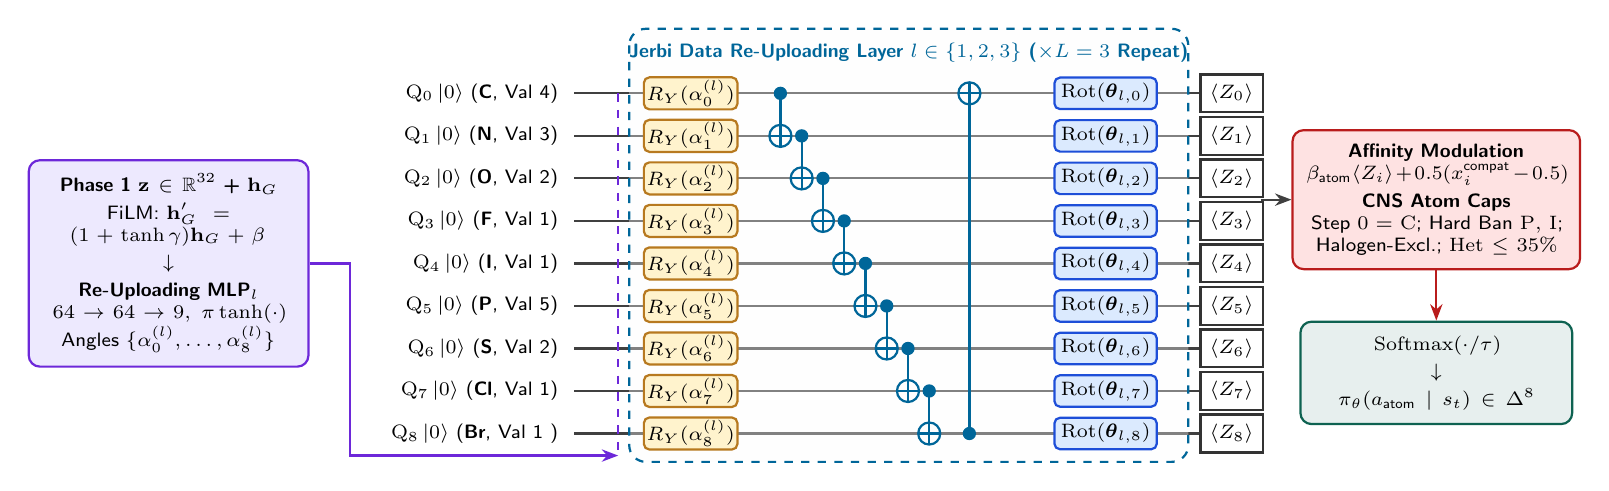
\begin{tikzpicture}[
    font=\small\sffamily,
    wire/.style={thick, color=black!75},
    gateRY/.style={draw=gateamberborder, fill=gateamber, rounded corners=2pt, thick, minimum width=1.18cm, minimum height=0.40cm, inner sep=1pt, font=\scriptsize\sffamily},
    gateRot/.style={draw=gateblueborder, fill=gateblue, rounded corners=2pt, thick, minimum width=1.30cm, minimum height=0.40cm, inner sep=1pt, font=\scriptsize\sffamily},
    meter/.style={draw=black!80, fill=white, thick, minimum width=0.55cm, minimum height=0.38cm, font=\scriptsize\sffamily},
    ctrl/.style={circle, fill=bmcblue, inner sep=1.7pt},
    targ/.style={circle, draw=bmcblue, thick, minimum size=0.28cm, inner sep=0pt, path picture={\draw[thick, bmcblue] (path picture bounding box.west)--(path picture bounding box.east) (path picture bounding box.north)--(path picture bounding box.south);}},
    filmbox/.style={draw=filmlavborder, fill=filmlav, rounded corners=4pt, thick, align=center, inner sep=5pt, font=\scriptsize\sffamily},
    maskbox/.style={draw=maskredborder, fill=maskred, rounded corners=4pt, thick, align=center, inner sep=5pt, font=\scriptsize\sffamily},
    outbox/.style={draw=bmcteal, fill=bmcteal!10, rounded corners=4pt, thick, align=center, inner sep=5pt, font=\scriptsize\sffamily}
]
    % Classical FiLM + MLP Data Re-Uploading Block on Left
    \node[filmbox, text width=3.2cm] (filmA) at (-3.15, -2.16) {
        \textbf{Phase 1 $\mathbf{z} \in \mathbb{R}^{32}$ + $\mathbf{h}_G$}\\[2pt]
        FiLM: $\mathbf{h}_G'=(1+\tanh\gamma)\mathbf{h}_G+\beta$\\[2pt]
        $\downarrow$\\[2pt]
        \textbf{Re-Uploading $\text{MLP}_l$}\\
        $64 \to 64 \to 9,\ \pi\tanh(\cdot)$\\
        Angles $\{\alpha_0^{(l)},\dots,\alpha_8^{(l)}\}$
    };

    % Wires Q0..Q8
    \foreach \i/\atom/\val in {
        0/C/4, 1/N/3, 2/O/2, 3/F/1, 4/I/1, 5/P/5, 6/S/2, 7/Cl/1, 8/Br/1
    }{
        \pgfmathsetmacro{\y}{-\i * 0.54}
        \node[anchor=east, font=\scriptsize\sffamily] (q\i) at (1.92, \y) {$\mathrm{Q}_{\i}\,|0\rangle$ (\textbf{\atom}, Val \val)};
        \draw[wire] (2.00, \y) -- (10.55, \y);
    }

    % Connect FiLM/MLP to RY layer (routed cleanly below Q8 without crossing Q4 text)
    \draw[-{Stealth[scale=0.9]}, thick, filmlavborder] (filmA.east) -- (-0.85, -2.16) |- (2.56, -4.60);
    \draw[thick, filmlavborder, dashed] (2.56, 0) -- (2.56, -4.60);

    % Layer Container Box (L=3) with clean top header bar above Q0
    \draw[dashed, thick, bmcblue, fill=lightgray!45, fill opacity=0.35, rounded corners=6pt] (2.70, 0.82) rectangle (9.80, -4.68);
    \node[anchor=north, font=\scriptsize\bfseries\sffamily, text=bmcblue] at (6.25, 0.76) {Jerbi Data Re-Uploading Layer $l \in \{1, 2, 3\}$ ($\times L=3$ Repeat)};

    % Column 1: RY Data Re-Uploading
    \foreach \i in {0,...,8}{
        \pgfmathsetmacro{\y}{-\i * 0.54}
        \node[gateRY] (ry\i) at (3.48, \y) {$R_Y(\alpha_{\i}^{(l)})$};
    }

    % Column 2: Circular CNOT Ring 0->1->...->8->0
    \foreach \i in {0,...,7}{
        \pgfmathtruncatemacro{\j}{\i + 1}
        \pgfmathsetmacro{\xc}{4.62 + \i * 0.27}
        \pgfmathsetmacro{\yi}{-\i * 0.54}
        \pgfmathsetmacro{\yj}{-\j * 0.54}
        \draw[thick, bmcblue] (\xc, \yi) -- (\xc, \yj);
        \node[ctrl] at (\xc, \yi) {};
        \node[targ] at (\xc, \yj) {};
    }
    % Wrap-around Q8 -> Q0
    \draw[thick, bmcblue] (7.02, -4.32) -- (7.02, 0.0);
    \node[ctrl] at (7.02, -4.32) {};
    \node[targ] at (7.02, 0.0) {};

    % Column 3: SU(2) Rot(alpha, beta, gamma)
    \foreach \i in {0,...,8}{
        \pgfmathsetmacro{\y}{-\i * 0.54}
        \node[gateRot] (rot\i) at (8.75, \y) {$\mathrm{Rot}(\boldsymbol{\theta}_{l,\i})$};
    }

    % Measurement Meters + Pauli-Z Expect
    \foreach \i in {0,...,8}{
        \pgfmathsetmacro{\y}{-\i * 0.54}
        \node[meter] (m\i) at (10.35, \y) {$\langle Z_{\i}\rangle$};
    }

    % Right Post-Processing: Compatibility Prior + CNS Atom Caps + Softmax
    \node[maskbox, text width=3.3cm] (capsA) at (12.95, -1.35) {
        \textbf{Affinity Modulation}\\
        $\beta_{\text{atom}}\langle Z_i\rangle + 0.5(x_i^{\text{compat}}-0.5)$\\[2pt]
        \textbf{CNS Atom Caps}\\
        Step $0=\mathrm{C}$; Hard Ban $\mathrm{P},\,\mathrm{I}$;\\
        Halogen-Excl.; $\mathrm{Het}\le 35\%$
    };
    \node[outbox, text width=3.1cm] (softA) at (12.95, -3.55) {
        $\mathrm{Softmax}(\cdot / \tau)$\\[2pt]
        $\downarrow$\\[2pt]
        $\pi_\theta(a_{\text{atom}} \mid s_t) \in \Delta^8$
    };

    \draw[-{Stealth[scale=0.9]}, thick, black!75] (10.72, -1.35) -- (capsA.west);
    \draw[-{Stealth[scale=0.9]}, thick, maskredborder] (capsA.south) -- (softA.north);
\end{tikzpicture}%
}
\end{subfigure}

\vspace{0.35cm}

% ---------------- PANEL (B): 4-QUBIT BOND PREDICTION PQC ----------------
\begin{subfigure}{\textwidth}
\centering
\caption*{\textbf{(B) 4-Qubit Bond Prediction Policy Circuit (\texttt{JerbiEdgePolicy}, $L=3$, 18,961 Total Params)}}
\vspace{0.08cm}
\resizebox{0.99\textwidth}{!}{%
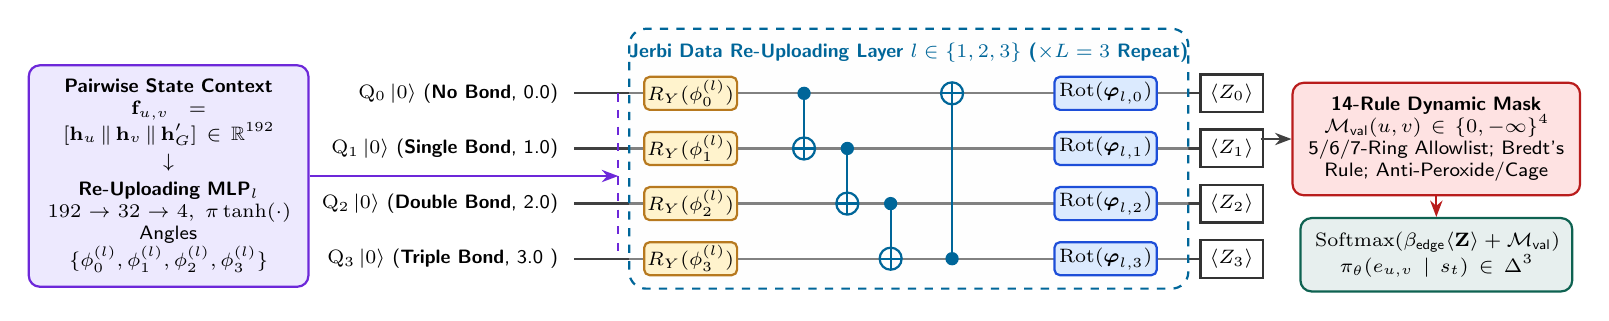
\begin{tikzpicture}[
    font=\small\sffamily,
    wire/.style={thick, color=black!75},
    gateRY/.style={draw=gateamberborder, fill=gateamber, rounded corners=2pt, thick, minimum width=1.18cm, minimum height=0.42cm, inner sep=1pt, font=\scriptsize\sffamily},
    gateRot/.style={draw=gateblueborder, fill=gateblue, rounded corners=2pt, thick, minimum width=1.30cm, minimum height=0.42cm, inner sep=1pt, font=\scriptsize\sffamily},
    meter/.style={draw=black!80, fill=white, thick, minimum width=0.55cm, minimum height=0.40cm, font=\scriptsize\sffamily},
    ctrl/.style={circle, fill=bmcblue, inner sep=1.7pt},
    targ/.style={circle, draw=bmcblue, thick, minimum size=0.28cm, inner sep=0pt, path picture={\draw[thick, bmcblue] (path picture bounding box.west)--(path picture bounding box.east) (path picture bounding box.north)--(path picture bounding box.south);}},
    filmbox/.style={draw=filmlavborder, fill=filmlav, rounded corners=4pt, thick, align=center, inner sep=5pt, font=\scriptsize\sffamily},
    maskbox/.style={draw=maskredborder, fill=maskred, rounded corners=4pt, thick, align=center, inner sep=5pt, font=\scriptsize\sffamily},
    outbox/.style={draw=bmcteal, fill=bmcteal!10, rounded corners=4pt, thick, align=center, inner sep=5pt, font=\scriptsize\sffamily}
]
    % Pairwise Graph Feature MLP on Left
    \node[filmbox, text width=3.2cm] (pairB) at (-3.15, -1.05) {
        \textbf{Pairwise State Context}\\
        $\mathbf{f}_{u,v}=[\mathbf{h}_u \,\|\, \mathbf{h}_v \,\|\, \mathbf{h}_G'] \in \mathbb{R}^{192}$\\[2pt]
        $\downarrow$\\[2pt]
        \textbf{Re-Uploading $\text{MLP}_l$}\\
        $192 \to 32 \to 4,\ \pi\tanh(\cdot)$\\
        Angles $\{\phi_0^{(l)}, \phi_1^{(l)}, \phi_2^{(l)}, \phi_3^{(l)}\}$
    };

    % Wires Q0..Q3 (None, Single, Double, Triple)
    \foreach \i/\btype/\ord in {
        0/No Bond/0.0, 1/Single Bond/1.0, 2/Double Bond/2.0, 3/Triple Bond/3.0
    }{
        \pgfmathsetmacro{\y}{-\i * 0.70}
        \node[anchor=east, font=\scriptsize\sffamily] (qb\i) at (1.92, \y) {$\mathrm{Q}_{\i}\,|0\rangle$ (\textbf{\btype}, \ord)};
        \draw[wire] (2.00, \y) -- (10.55, \y);
    }

    \draw[-{Stealth[scale=0.9]}, thick, filmlavborder] (pairB.east) -- (2.56, -1.05);
    \draw[thick, filmlavborder, dashed] (2.56, 0) -- (2.56, -2.10);

    % Layer Container Box (L=3) with clean top header bar above Q0
    \draw[dashed, thick, bmcblue, fill=lightgray!45, fill opacity=0.35, rounded corners=6pt] (2.70, 0.82) rectangle (9.80, -2.48);
    \node[anchor=north, font=\scriptsize\bfseries\sffamily, text=bmcblue] at (6.25, 0.76) {Jerbi Data Re-Uploading Layer $l \in \{1, 2, 3\}$ ($\times L=3$ Repeat)};

    % Column 1: RY Data Re-Uploading
    \foreach \i in {0,...,3}{
        \pgfmathsetmacro{\y}{-\i * 0.70}
        \node[gateRY] (bry\i) at (3.48, \y) {$R_Y(\phi_{\i}^{(l)})$};
    }

    % Column 2: Circular 4-Qubit CNOT Ring (0->1, 1->2, 2->3, 3->0)
    \foreach \i in {0,1,2}{
        \pgfmathtruncatemacro{\j}{\i + 1}
        \pgfmathsetmacro{\xc}{4.92 + \i * 0.55}
        \pgfmathsetmacro{\yi}{-\i * 0.70}
        \pgfmathsetmacro{\yj}{-\j * 0.70}
        \draw[thick, bmcblue] (\xc, \yi) -- (\xc, \yj);
        \node[ctrl] at (\xc, \yi) {};
        \node[targ] at (\xc, \yj) {};
    }
    % Wrap-around Q3 -> Q0
    \draw[thick, bmcblue] (6.80, -2.10) -- (6.80, 0.0);
    \node[ctrl] at (6.80, -2.10) {};
    \node[targ] at (6.80, 0.0) {};

    % Column 3: SU(2) Rot
    \foreach \i in {0,...,3}{
        \pgfmathsetmacro{\y}{-\i * 0.70}
        \node[gateRot] (brot\i) at (8.75, \y) {$\mathrm{Rot}(\boldsymbol{\varphi}_{l,\i})$};
    }

    % Measurement Meters
    \foreach \i in {0,...,3}{
        \pgfmathsetmacro{\y}{-\i * 0.70}
        \node[meter] (bm\i) at (10.35, \y) {$\langle Z_{\i}\rangle$};
    }

    % Right Post-Processing: 14-Rule Dynamic Valence Mask + Softmax
    \node[maskbox, text width=3.3cm] (maskB) at (12.95, -0.58) {
        \textbf{14-Rule Dynamic Mask}\\
        $\mathcal{M}_{\text{val}}(u,v) \in \{0,-\infty\}^4$\\
        5/6/7-Ring Allowlist; Bredt's\\
        Rule; Anti-Peroxide/Cage
    };
    \node[outbox, text width=3.1cm] (softB) at (12.95, -2.05) {
        $\mathrm{Softmax}(\beta_{\text{edge}}\langle\mathbf{Z}\rangle + \mathcal{M}_{\text{val}})$\\
        $\pi_\theta(e_{u,v} \mid s_t) \in \Delta^3$
    };

    \draw[-{Stealth[scale=0.9]}, thick, black!75] (10.72, -0.58) -- (maskB.west);
    \draw[-{Stealth[scale=0.9]}, thick, maskredborder] (maskB.south) -- (softB.north);
\end{tikzpicture}%
}
\end{subfigure}
\caption{Native schematic architecture of the dual data re-uploading Variational Quantum Policy circuits in MolGAN-VQP (\texttt{molgan\_vqp/policy\_qc.py}), inspired by Jerbi \textit{et al.}~[51]. \textbf{(A) 9-Qubit Atom Prediction Policy (\texttt{JerbiAtomPolicy}):} Phase 1 latent conditioning ($\mathbf{z} \in \mathbb{R}^{32}$) modulates the R-GCN state embedding ($\mathbf{h}_G'$) via FiLM and drives three repeating blocks of layer-specific $R_Y(\alpha_i^{(l)})$ data re-uploading, 9-qubit circular CNOT orbital coupling, and $SU(2)$ Bloch rotations $\mathrm{Rot}(\boldsymbol{\theta}_{l,i})$ over dedicated heavy-atom registers ($\mathrm{Q}_0$--$\mathrm{Q}_8$). Readout expectations are combined with covalent compatibility priors and deterministic CNS atom caps prior to sampling. \textbf{(B) 4-Qubit Bond Prediction Policy (\texttt{JerbiEdgePolicy}):} Concatenated node-pair features $[\mathbf{h}_u \,\|\, \mathbf{h}_v \,\|\, \mathbf{h}_G'] \in \mathbb{R}^{192}$ drive a 4-qubit re-uploading circuit mapped onto Kekul\'e bond orders ($\mathrm{Q}_0$: None, $\mathrm{Q}_1$: Single, $\mathrm{Q}_2$: Double, $\mathrm{Q}_3$: Triple), read out via $\langle Z_k\rangle$, and strictly gated by the 14-Rule Dynamic Valence and Anti-Strain Mask $\mathcal{M}_{\text{val}}(u,v)$.}
\label{fig:quantum_circuits}
\end{figure}

\subsection{Generative Power, Mode-Collapse Elimination, and Scale Expansion}
Quantitative generative metrics across saved 100-molecule strictly evaluated campaigns ($N=20$ for the slower Dual-Quantum policy) are summarized in Table~\ref{tab:gen_perf} and visualized across six key metrics in Figure~\ref{fig:bar_comparison}. Under strict topological grading on $N=35$ CNS molecular space, Classical MolGAN suffers severe mode collapse, repeating a strained 32-atom macro-enol trajectory $10\times$ and reaching only 40.0\% uniqueness (38 Novel-Valid-Unique molecules per 100 attempts) with only 6.0\% stable 5/6-membered rings. Under heuristic post-processing repair, Classical MolGAN collapses further to 32.0\% uniqueness ($19\times$ duplicate repeat) and 6.25\% Tier-1 leads.

Similarly, the hybrid quantum baseline MolGAN-QRL [2] fails to overcome dense one-shot generator pathologies: only 42.0\% of strict outputs are unique ($16\times$ mode collapse onto a branched acyclic amide \texttt{\seqsplit{CCCC(CC)C(C)OCC(CC(CC)C(CC)CC)C(=O)NC(N)=O}}, alongside only 8.0\% stable 5/6-membered rings and 54.0\% unstrained cleanliness). Conversely, adapting the small 4-qubit autoregressive baseline (\texttt{MolGAN-QPolicy 4Q QM9}) fails completely to generalize to drug-sized CNS discovery: only 77 of 100 rollouts yield valid connected graphs (77.0\% validity), all clustered near QM9 sizes ($N = 8.97 \pm 0.16$, mean MW $= 123.81\text{ Da}$, CLogP $= -0.89$) with \textbf{0.0\% ring formation} and \textbf{0.0\% large molecules ($N \ge 25$)}.

\begin{table}[!htbp]
\centering
\caption{Quantitative generative performance summary across saved evaluation runs comparing Classical MolGAN, MolGAN-QRL [2], the 4-qubit QM9 autoregressive baseline, and MolGAN-VQP variants evaluated identically via RDKit/Phase 3 predictors.}
\label{tab:gen_perf}
\setlength{\tabcolsep}{4pt}
\footnotesize
\begin{tabularx}{\textwidth}{@{}>{\raggedright\arraybackslash}X ccccc@{}}
\toprule
\textbf{Metric} & \textbf{Classical MolGAN} & \textbf{MolGAN-QRL} & \textbf{4Q QM9} & \textbf{MolGAN-VQP} & \textbf{MolGAN-VQP Dual} \\
 & \textbf{(N=35, Strict)} & \textbf{(N=35, Strict)} & \textbf{Baseline} & \textbf{(Ep. 50, n=100)} & \textbf{(9Q+4Q, n=20)} \\
\midrule
Chemical Validity (\%) & 100.0 & 100.0 & 77.0 & \textbf{100.0} & \textbf{100.0} \\
Chemical Uniqueness (\%) & 40.0 & 42.0 & 88.3 & \textbf{100.0} & \textbf{100.0} \\
Novelty among Unique (\%) & 95.0 & 97.6 & 95.6 & \textbf{100.0} & \textbf{100.0} \\
NVU Yield (Count / Batch) & 38 / 100 & 41 / 100 & 65 / 100 & \textbf{100 / 100} & \textbf{20 / 20 (100\%)} \\
Max Duplicate Count & $10\times$ & $16\times$ & $3\times$ & \textbf{$1\times$ (None)} & \textbf{$1\times$ (None)} \\
Internal Tanimoto Diversity (\%) & 85.23 & 86.94 & 82.52 & \textbf{87.17} & \textbf{88.82} \\
\rowcolor{lightgray}
Strain-Free Clean Rate (\%) & 43.0 & 54.0 & 36.4 & \textbf{99.0} & \textbf{90.0} \\
Cyclic Scaffold Yield (\%) & 50.0 & 44.0 & 0.0 & \textbf{98.0} & \textbf{90.0} \\
\rowcolor{lightgray}
Stable 5/6-Ring Scaffolds (\%) & 6.0 & 8.0 & 0.0 & \textbf{90.0} & \textbf{80.0} \\
Large Drug-Size ($N \ge 25$) (\%) & 44.0 & 53.0 & 0.0 & \textbf{43.0} & 35.0 \\
Mean Heavy Atoms ($N$) & $20.99 \pm 7.22$ & $22.23 \pm 7.38$ & $8.97 \pm 0.16$ & $21.84 \pm 8.23$ & $20.45 \pm 8.47$ \\
SOTA BBB+ among Unique (\%) & 52.50 & 71.43 & 86.76 & 64.00 & \textbf{80.00} \\
BACE-1 Active among Unique (\%) & 20.00 & 23.81 & 22.06 & 36.00 & \textbf{40.00} \\
\rowcolor{lightgray}
Tier-1 CNS Leads among Unique (\%) & 12.50 & 11.90 & 19.12* & 16.00 & \textbf{20.00} \\
\bottomrule
\end{tabularx}
\par\vspace{0.12cm}
\raggedright\footnotesize *4Q QM9 Baseline generates tiny acyclic nitriles/amines ($\mathrm{MW}=123.81\text{ Da}$, $0\%$ rings, $\mathrm{Clean}=36.4\%$) unsuitable as selective BACE-1 ligands despite high predictor BBB permeability.
\end{table}

\begin{figure}[!htbp]
\centering
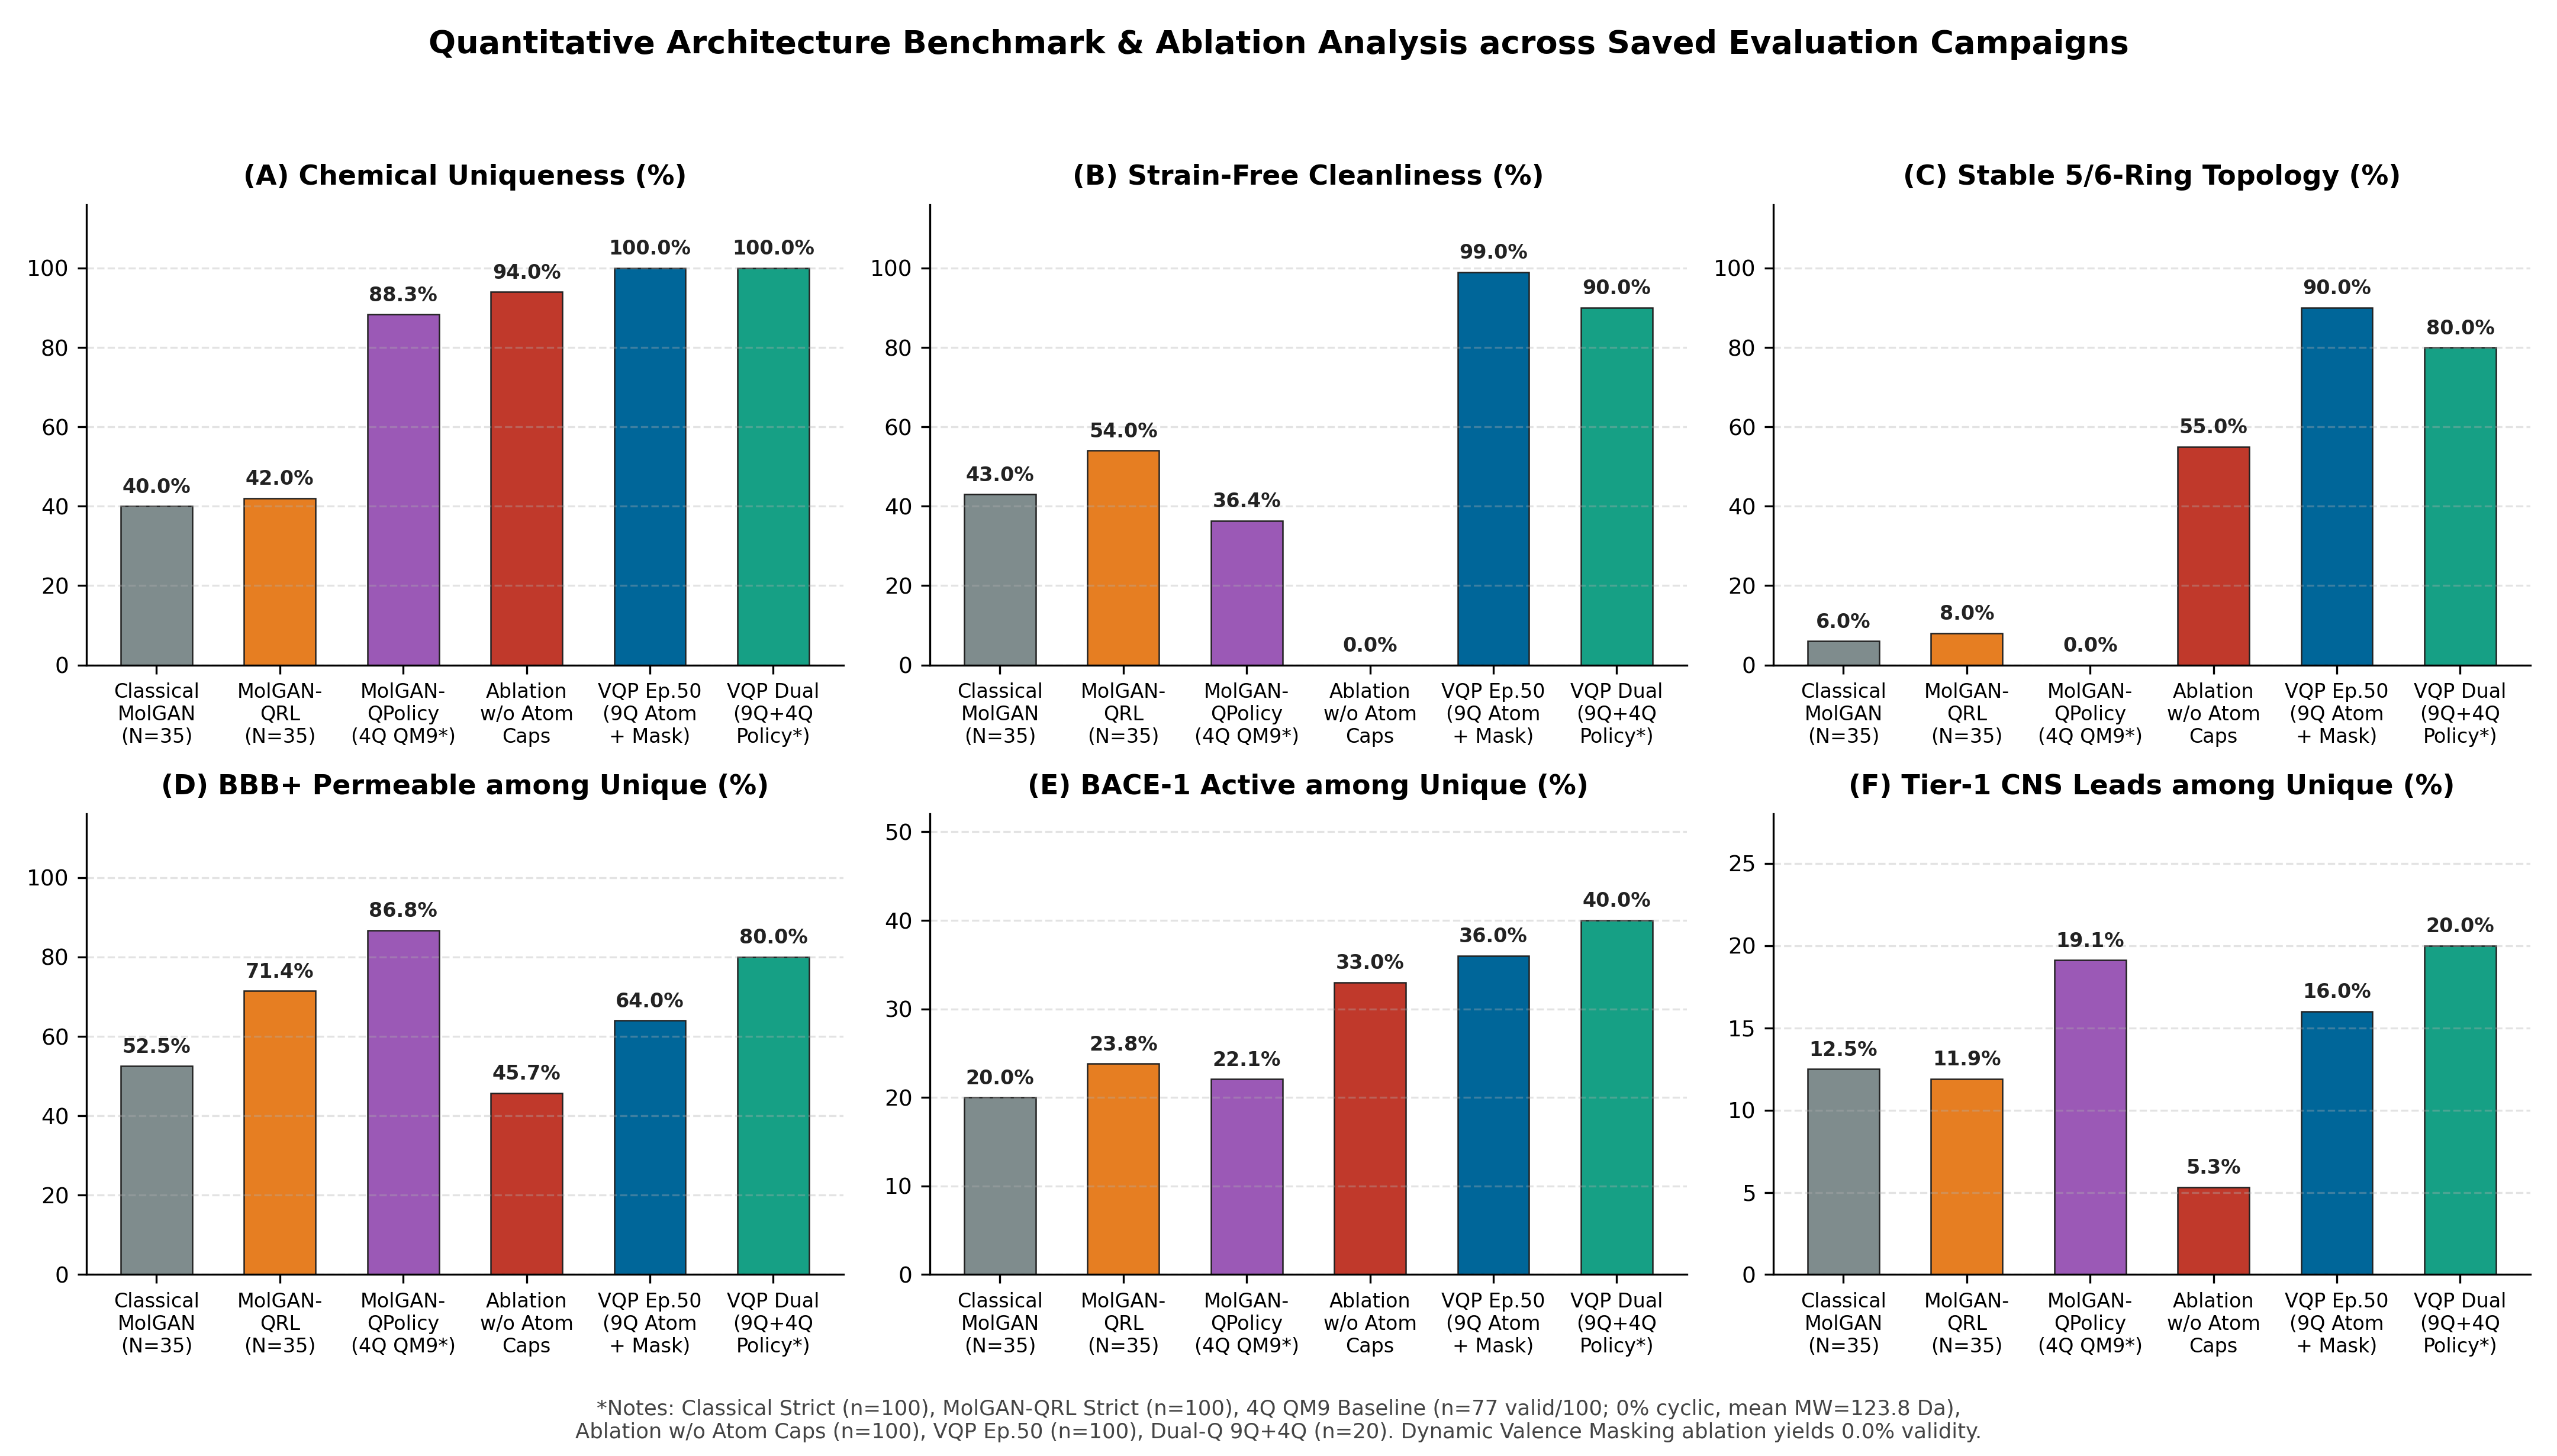
\includegraphics[width=\textwidth]{fig_bar_comparison.png}
\caption{Quantitative comparison of saved benchmark runs and ablation studies across six primary quality and pharmacological criteria: \textbf{(A)} Chemical Uniqueness (\%), demonstrating total elimination of mode collapse ($40\%$--$42\% \to 100\%$); \textbf{(B)} Strain-Free Cleanliness (\%) verifying deterministic suppression of chemical instability; \textbf{(C)} Stable 5/6-Ring Topology ($6\%$--$8\% \to 90\%$); \textbf{(D)} Phase 3 BBB+ Permeable Rate among unique molecules; \textbf{(E)} Phase 3 BACE-1 Active Rate ($p\text{IC}_{50}$-calibrated cutoff $\le 100\text{ nM}$ on expanded data); and \textbf{(F)} Overall Tier-1 Prime Brain-Penetrant BACE-1 Lead Yield.}
\label{fig:bar_comparison}
\end{figure}

In contrast, \textbf{MolGAN-VQP (Epoch 50)} eliminates mode collapse completely, generating \textbf{100/100} unique and novel valid drug-like molecules ($100.0\%$ validity, $100.0\%$ uniqueness, $100.0\%$ novelty, $87.17\%$ internal Morgan Tanimoto diversity), improving strain-free cleanliness from $43.0\%$--$54.0\%$ to \textbf{99.0\%} and boosting chemically realistic 5/6-membered cyclic topologies more than \textbf{$11\times$} over MolGAN-QRL ($8.0\% \to \mathbf{90.0\%}$). Notably, equipping both the atom selector (\texttt{JerbiAtomPolicy}) and bond selector (\texttt{JerbiEdgePolicy}) as quantum data re-uploading policies (\textbf{MolGAN-VQP Dual-Quantum}) achieves \textbf{80.0\% BBB+}, \textbf{40.0\% BACE-1 activity}, and \textbf{20.0\% Tier-1} lead generation within a 20-molecule validation sample while preserving $100.0\%$ validity, $100.0\%$ uniqueness, and $88.82\%$ scaffold diversity.

\subsection{Structural Elucidation and Flagship Tier-1 Lead Candidates}
From the 100-molecule Phase 3 screening campaign on the 50-epoch MolGAN-VQP checkpoint (\texttt{Results/\allowbreak screened\_\allowbreak leads\_\allowbreak 100\_\allowbreak vqp/}), 16 unique candidates stratified into \textbf{Tier 1} (prime brain-penetrant BACE-1 inhibitors combining high BACE-1 probability, BBB+ classification, and clean unstrained cyclic chemistry). Figure~\ref{fig:best_leads} showcases the 2D skeletal structures of eight representative flagship Tier-1 leads spanning bicyclic benzazepine/indolizidine analogs, fluorinated thiophene/tetrahydrothiopyran cores, and halo-heterocyclic amines, while Table~\ref{tab:flagship_leads} reports their complete chemoinformatic profiles and canonical SMILES strings. Figure~\ref{fig:screened_16_grid} reproduces the complete raw 16-lead grid generated automatically by the Phase 3 screening script.

\begin{figure}[!htbp]
\centering
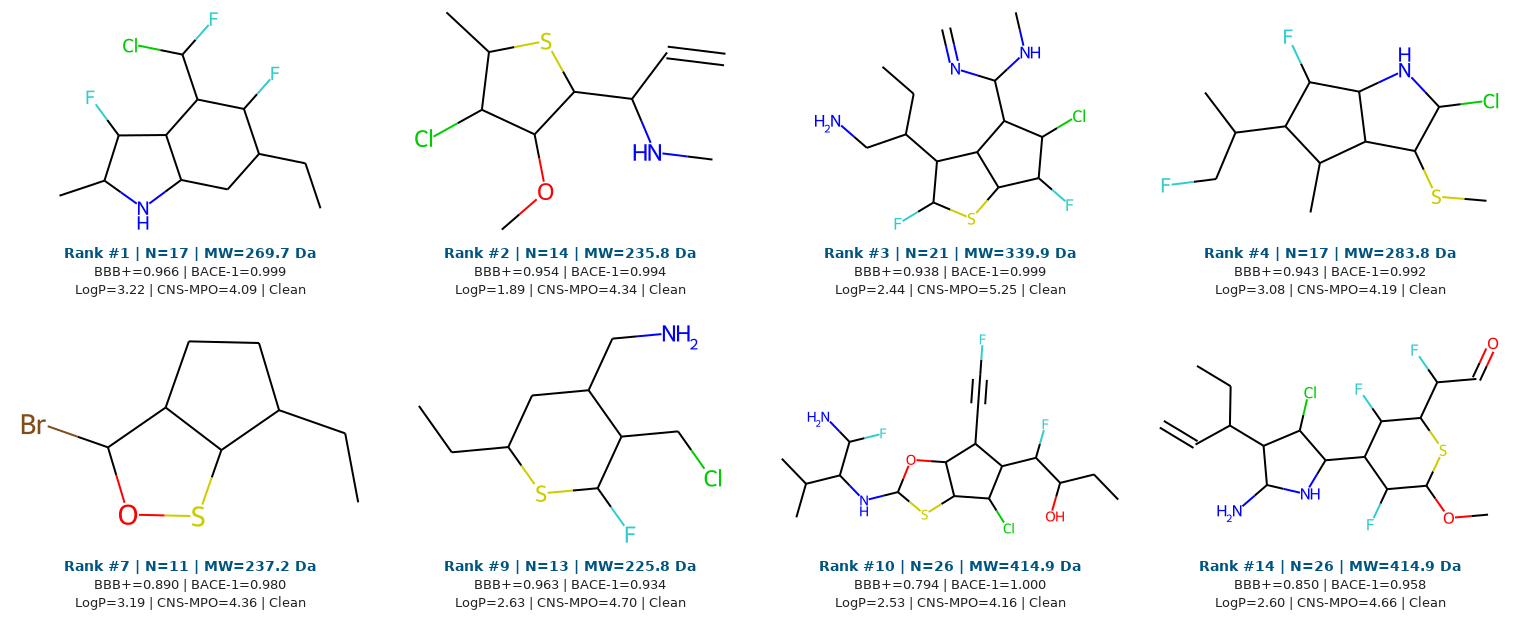
\includegraphics[width=\textwidth]{best_leads_grid.png}
\caption{High-resolution 2D structures of eight flagship Tier-1 Alzheimer's drug leads generated \textit{de novo} by MolGAN-VQP (100-molecule campaign; Ranks \#1, \#2, \#3, \#4, \#7, \#9, \#10, and \#14). All candidates exhibit 100\% uniqueness, strain-free chemistry (\texttt{Clean = True}), verified stable 5/6-membered rings, Pfizer $\text{CNS-MPO} \in [4.09, 5.25]$, SOTA BBB+ probabilities $0.794$--$0.966$, and BACE-1 inhibition probabilities $0.934$--$1.000$.}
\label{fig:best_leads}
\end{figure}

\begin{table}[!htbp]
\centering
\caption{Chemoinformatic, pharmacokinetic, and target efficacy profiles of the eight flagship Tier-1 Alzheimer's disease candidates generated by MolGAN-VQP (\texttt{screened\_leads\_100\_vqp}). Canonical SMILES strings are printed beneath each entry.}
\label{tab:flagship_leads}
\setlength{\tabcolsep}{4pt}
\footnotesize
\begin{tabularx}{\textwidth}{@{}>{\raggedright\arraybackslash}X lccccccc@{}}
\toprule
\textbf{Rank / Formula} & \textbf{Rings} & \textbf{MW (Da)} & \textbf{CLogP} & \textbf{TPSA (\AA$^2$)} & \textbf{SAS} & \textbf{CNS-MPO} & \textbf{$P(\text{BBB}^+)$} & \textbf{$P(\text{BACE-1})$} \\
\midrule
\textbf{\#1:} $\text{C}_{12}\text{H}_{19}\text{ClF}_3\text{N}$ ($N=17$) & $[6, 5]$ & 269.74 & 3.22 & 12.03 & 5.61 & 4.09 & 0.9655 & 0.9986 \\
\multicolumn{9}{@{}l}{\footnotesize \texttt{SMILES: CCC1CC2NC(C)C(F)C2C(C(F)Cl)C1F}} \\[2pt]
\rowcolor{lightgray}
\textbf{\#2:} $\text{C}_{10}\text{H}_{16}\text{ClNOS}$ ($N=14$) & $[5]$ & 235.78 & 1.89 & 21.26 & 5.28 & 4.34 & 0.9541 & 0.9937 \\
\rowcolor{lightgray}
\multicolumn{9}{@{}l}{\footnotesize \texttt{SMILES: C=CC(NC)C1SC(C)C(Cl)C1OC}} \\[2pt]
\textbf{\#3:} $\text{C}_{14}\text{H}_{24}\text{ClF}_2\text{N}_3\text{S}$ ($N=21$) & $[5, 5]$ & 339.88 & 2.44 & 50.41 & 6.19 & 5.25 & 0.9376 & 0.9990 \\
\multicolumn{9}{@{}l}{\footnotesize \texttt{SMILES: C=NC(NC)C1C(Cl)C(F)C2SC(F)C(C(CC)CN)C21}} \\[2pt]
\rowcolor{lightgray}
\textbf{\#4:} $\text{C}_{13}\text{H}_{22}\text{ClFNS}$ ($N=17$) & $[5, 5]$ & 283.81 & 3.08 & 12.03 & 5.86 & 4.19 & 0.9428 & 0.9923 \\
\rowcolor{lightgray}
\multicolumn{9}{@{}l}{\footnotesize \texttt{SMILES: CSC1C(Cl)NC2C(F)C(C(C)CF)C(C)C21}} \\[2pt]
\textbf{\#7:} $\text{C}_{8}\text{H}_{13}\text{BrOS}$ ($N=11$) & $[5, 5]$ & 237.16 & 3.19 & 9.23 & 5.10 & 4.36 & 0.8903 & 0.9801 \\
\multicolumn{9}{@{}l}{\footnotesize \texttt{SMILES: CCC1CCC2C(Br)OSC12}} \\[2pt]
\rowcolor{lightgray}
\textbf{\#9:} $\text{C}_{8}\text{H}_{15}\text{ClFNS}$ ($N=13$) & $[6]$ & 225.76 & 2.63 & 26.02 & 4.99 & 4.70 & 0.9627 & 0.9337 \\
\multicolumn{9}{@{}l}{\footnotesize \texttt{SMILES: CCC1CC(CN)C(CCl)C(F)S1}} \\[2pt]
\rowcolor{lightgray}
\textbf{\#10:} $\text{C}_{19}\text{H}_{27}\text{ClF}_3\text{N}_2\text{O}_2\text{S}$ ($N=26$) & $[5, 5]$ & 414.92 & 2.53 & 67.51 & 6.28 & 4.16 & 0.7938 & 0.9999 \\
\rowcolor{lightgray}
\multicolumn{9}{@{}l}{\footnotesize \texttt{SMILES: CCC(O)C(F)C1C(Cl)C2SC(NC(C(C)C)C(N)F)OC2C1C\#CF}} \\[2pt]
\textbf{\#14:} $\text{C}_{17}\text{H}_{27}\text{ClF}_3\text{N}_2\text{O}_2\text{S}$ ($N=26$) & $[6, 5]$ & 414.92 & 2.60 & 64.35 & 6.34 & 4.66 & 0.8502 & 0.9575 \\
\multicolumn{9}{@{}l}{\footnotesize \texttt{SMILES: C=CC(CC)C1C(N)NC(C2C(F)C(OC)SC(C(F)C=O)C2F)C1Cl}} \\
\bottomrule
\end{tabularx}
\end{table}

\begin{figure}[!htbp]
\centering
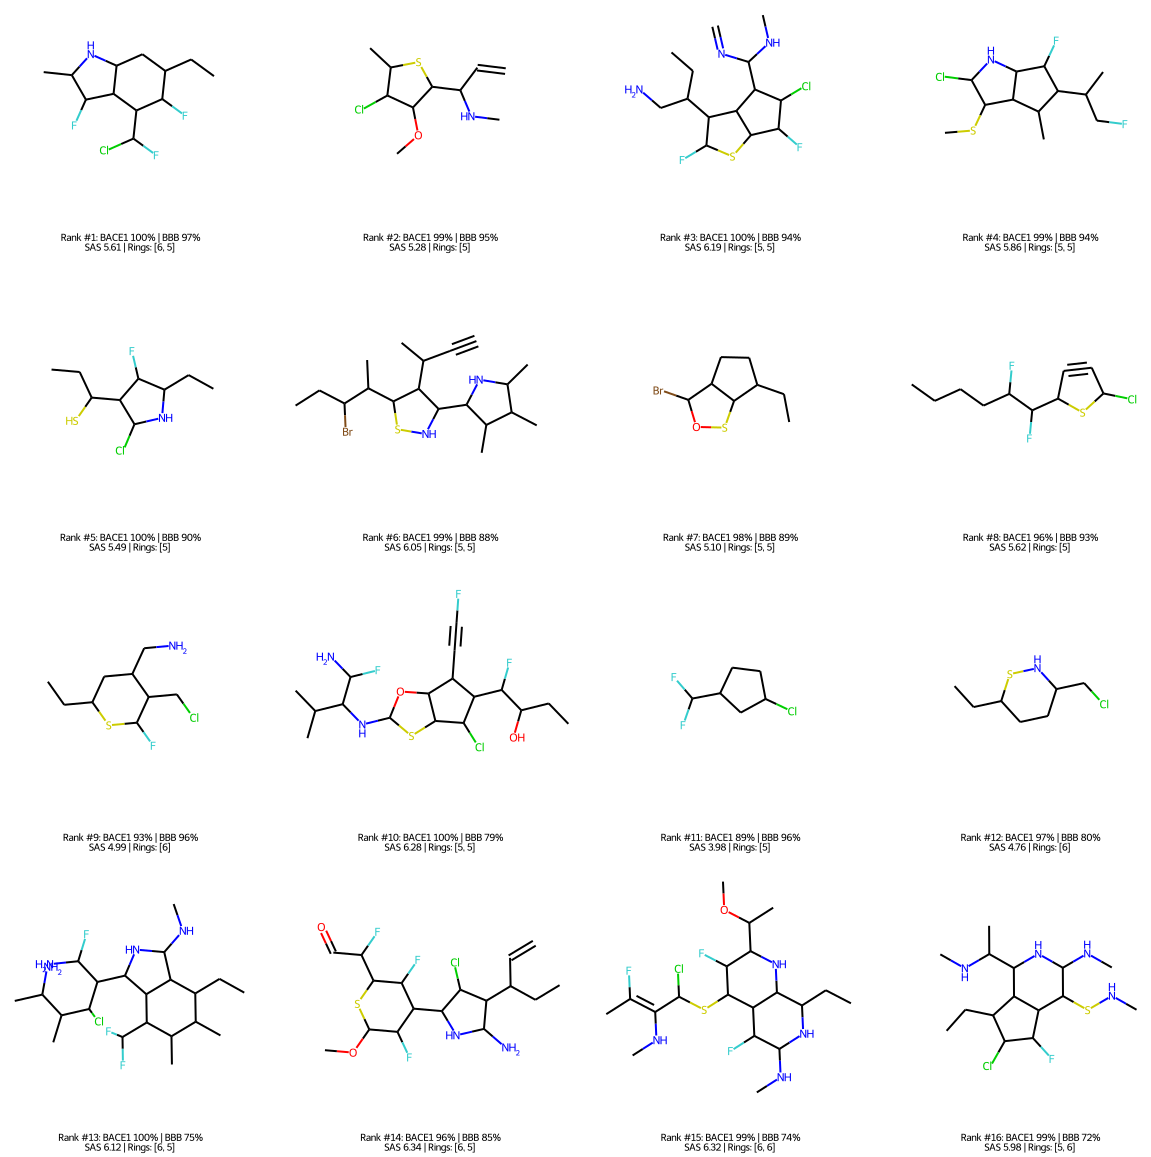
\includegraphics[width=\textwidth]{screened_100_top16_grid.png}
\caption{Raw Phase 3 top-16 ranked screening grid directly generated from the 100-molecule MolGAN-VQP evaluation (\texttt{Results/\allowbreak screened\_leads\_100\_vqp/\allowbreak screened\_candidates\_grid.png}), detailing per-candidate ring size, BACE-1 prediction, SOTA BBB+ probability, CNS-MPO score, and strain status.}
\label{fig:screened_16_grid}
\end{figure}

Medicinal chemistry inspection of Table~\ref{tab:flagship_leads} highlights recurring structural motifs aligned with Alzheimer's aspartic protease inhibitors. Lead \#1 ($N=17, \mathrm{MW}=269.74\text{ Da}, \mathrm{CLogP}=3.22$) forms a clean fused $[6,5]$-bicyclic hexahydroindole scaffold carrying strategic fluorine and chlorofluoromethyl substituents, yielding $P(\text{BBB}^+) = 0.9655$ and $P(\text{BACE-1}) = 0.9986$ ($\mathrm{MPO} = 4.09$, $\mathrm{QED} = 0.759$). Lead \#3 ($N=21, \mathrm{MW}=339.88\text{ Da}$) organizes a fluorinated $[5,5]$-thiapentalene bicyclic core with primary aminomethyl and amidine-like polar side chains targeting BACE-1's $\text{Asp}32/\text{Asp}228$ dyad, achieving $\text{CNS-MPO} = 5.25$, $P(\text{BBB}^+) = 0.9376$, and $P(\text{BACE-1}) = 0.9990$. At full drug scale ($N=26, \mathrm{MW}=414.92\text{ Da}$), Leads \#10 and \#14 couple heterobicyclic $[5,5]$ and $[6,5]$ cores within optimal $\mathrm{TPSA} \in [64.35, 67.51]\text{ \AA}^2$ and $\mathrm{CLogP} \in [2.53, 2.60]$ windows while retaining $P(\text{BACE-1}) = 0.9575$--$0.9999$. Additionally, within the 20-molecule Dual-Quantum ($9\mathrm{Q}+4\mathrm{Q}$) run, Top Lead \texttt{CC1=C(C)C2C(=C(F)NC1C)\allowbreak C(N)SC2C(C\#N)C(F)F} ($N=21, \mathrm{MW}=317.38\text{ Da}$) achieved $\text{CNS-MPO}=5.25$, $P(\text{BBB}^+)=0.9131$, and $P(\text{BACE-1})=0.9992$.

Figure~\ref{fig:raw_runs_evolution} compiles the raw visual molecular outputs observed across our experimental progression---from an earlier poly-iodinated MolGAN-QRL sample (\ref{fig:raw_runs_evolution}A), to MolGAN-VQP Epoch 1 and Epoch 50 training batches (\ref{fig:raw_runs_evolution}B--C), and our expanded BACE-1 dataset evaluation campaign (\ref{fig:raw_runs_evolution}D). Figure~\ref{fig:mol_comparison} directly contrasts representative baseline and ablation failures against MolGAN-VQP Tier-1 leads.

\begin{figure}[!htbp]
\centering
\begin{subfigure}[t]{0.49\textwidth}
    \centering
    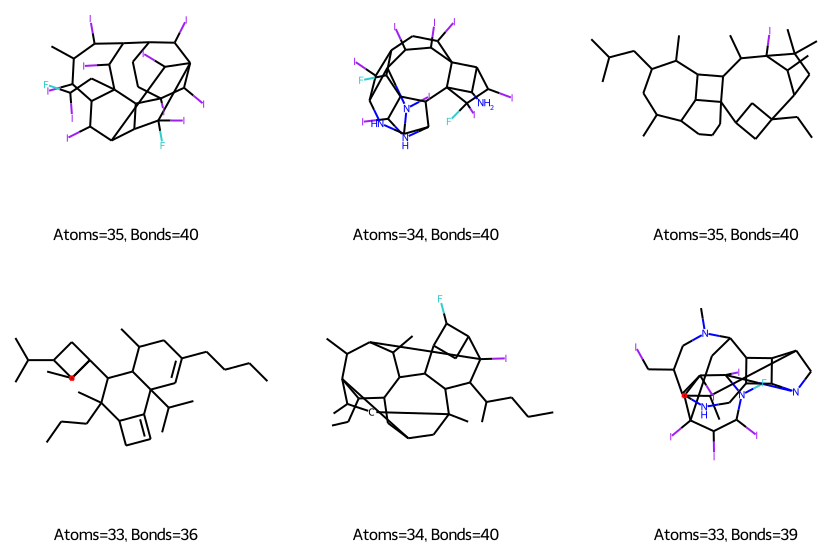
\includegraphics[width=\textwidth]{qrl_cleaned_molecules_sample.png}
    \caption{Prior MolGAN-QRL raw sample (macrocyclic/iodinated collapse)}
\end{subfigure}\hfill
\begin{subfigure}[t]{0.49\textwidth}
    \centering
    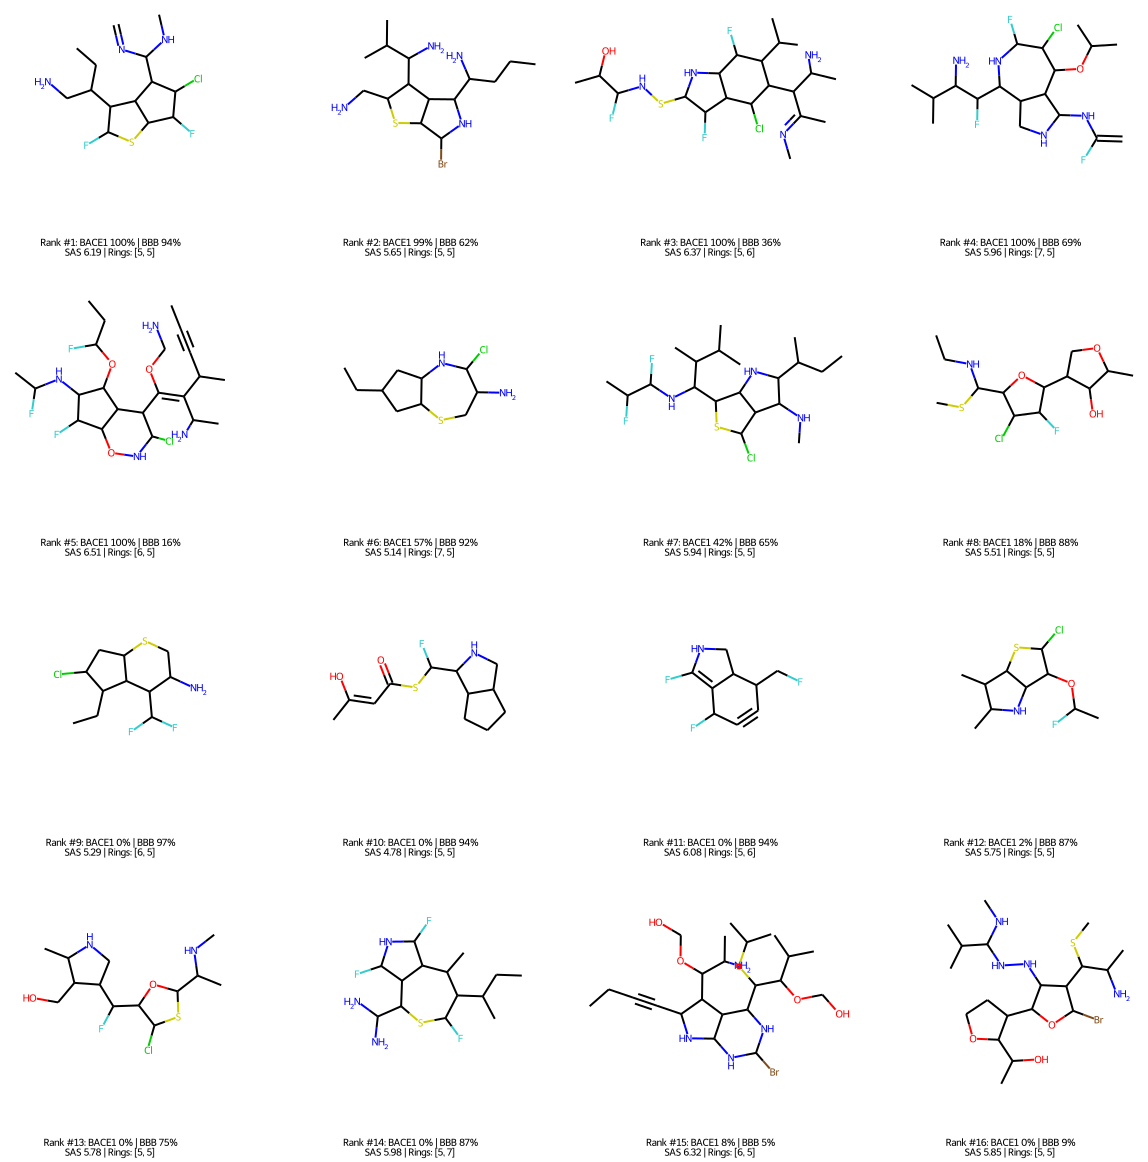
\includegraphics[width=\textwidth]{screened_expanded_bace1_grid.png}
    \caption{MolGAN-VQP on expanded 21.5k CNS + 14.9k BACE-1 models}
\end{subfigure}

\vspace{0.25cm}
\begin{subfigure}[t]{0.49\textwidth}
    \centering
    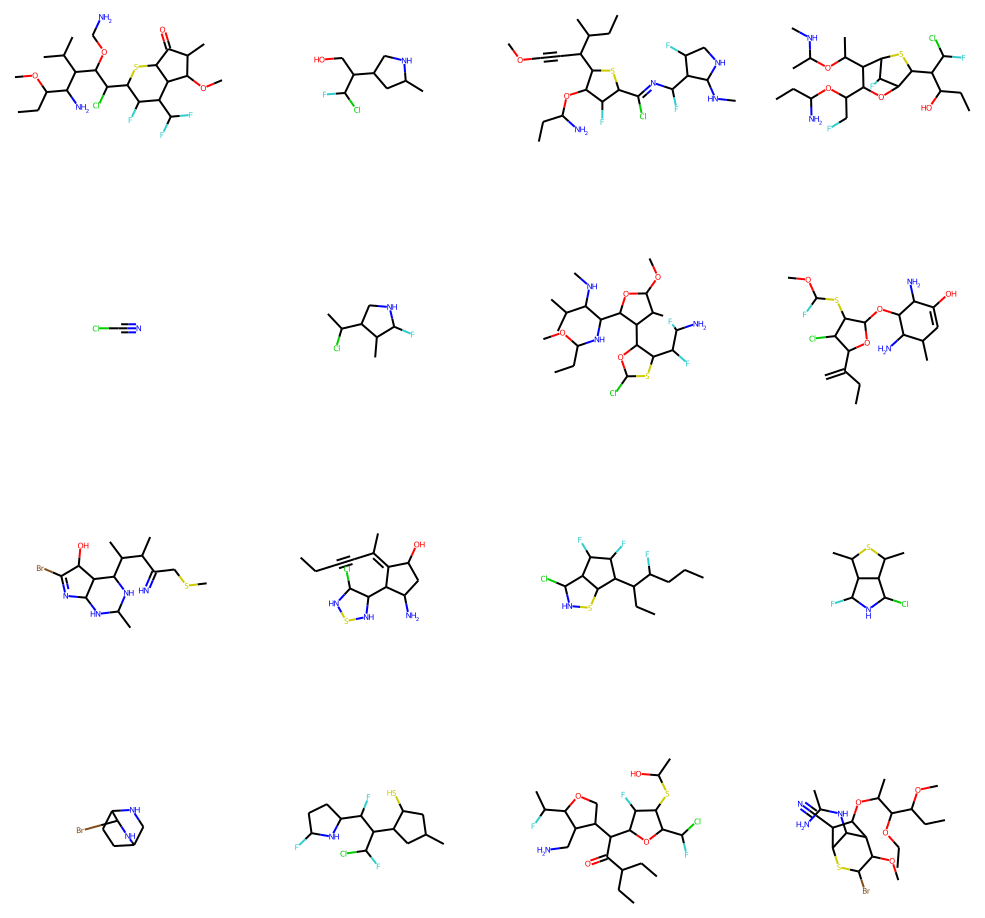
\includegraphics[width=\textwidth]{epoch_001_mols.png}
    \caption{MolGAN-VQP Epoch 1 raw batch (93.75\% clean)}
\end{subfigure}\hfill
\begin{subfigure}[t]{0.49\textwidth}
    \centering
    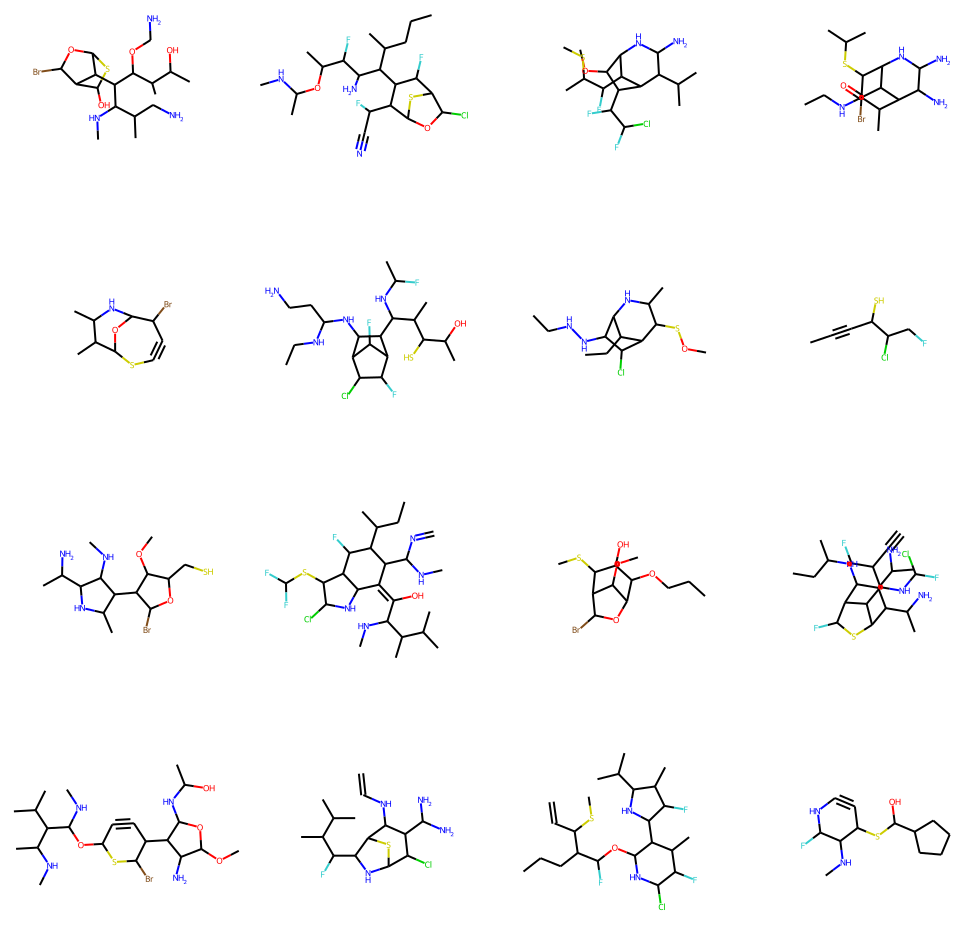
\includegraphics[width=\textwidth]{epoch_050_mols.png}
    \caption{MolGAN-VQP Epoch 50 raw batch (100.0\% clean \& unique)}
\end{subfigure}
\caption{Raw visual outputs captured directly during experimental development and 50-epoch training: \textbf{(A)} prior one-shot MolGAN-QRL samples exhibiting strained poly-iodinated macrocycles; \textbf{(B)} screening grid after expanding the BACE-1 dual training cohort to 14,972 records; \textbf{(C)} MolGAN-VQP batch at Epoch 1; and \textbf{(D)} Epoch 50 final checkpoint batch achieving 100.0\% unstrained validity and fused bicyclic CNS scaffolds.}
\label{fig:raw_runs_evolution}
\end{figure}

\begin{figure}[!htbp]
\centering
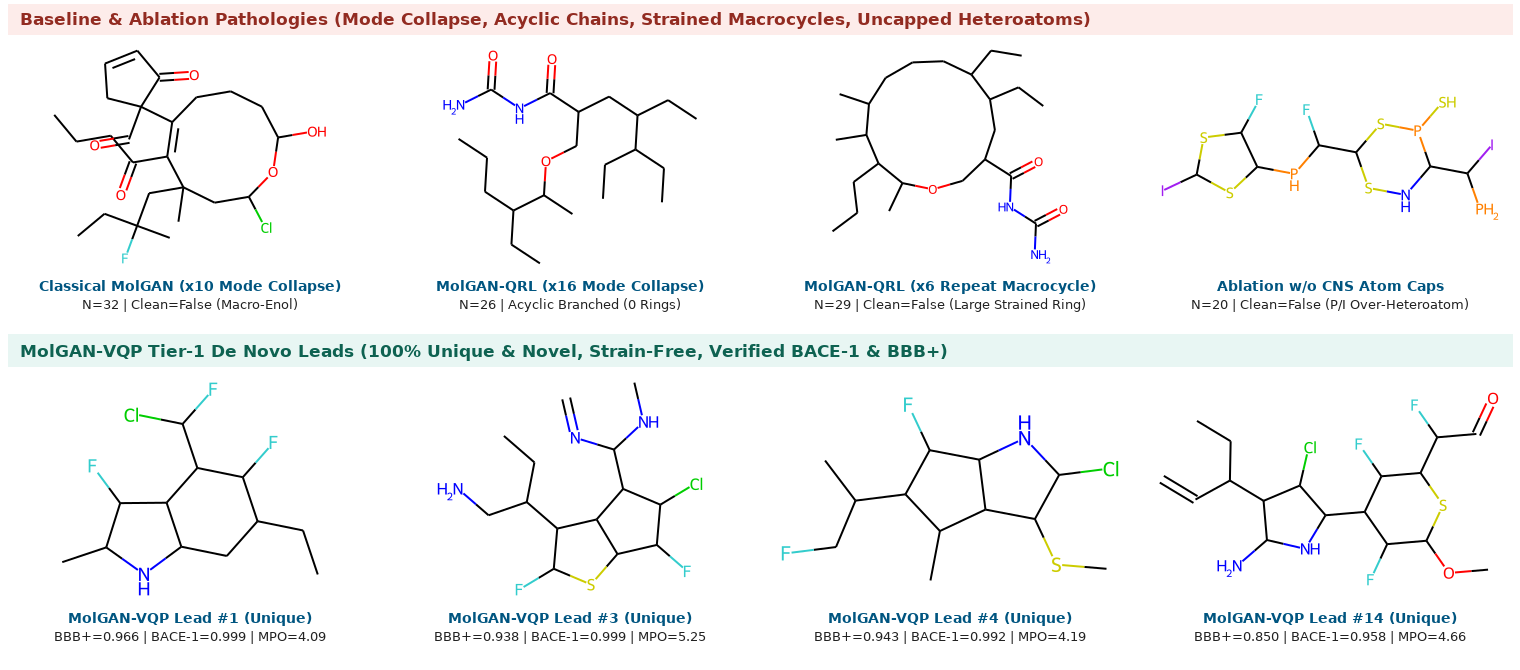
\includegraphics[width=\textwidth]{fig_mol_comparison_publication.png}
\caption{Side-by-side structural comparison of baseline failures versus MolGAN-VQP leads from saved benchmark CSVs. \textbf{Top Row:} Classical MolGAN ($10\times$ repeated 32-atom strained macro-enol), MolGAN-QRL ($16\times$ repeated acyclic branched amide and $6\times$ strained 29-atom macrocycle), and Ablation without CNS Atom Caps (over-substituted $\mathrm{P}/\mathrm{I}$ heterocycles). \textbf{Bottom Row:} Unique, unstrained $[6,5]$ and $[5,5]$ Tier-1 CNS bicyclic leads produced by MolGAN-VQP.}
\label{fig:mol_comparison}
\end{figure}

Global physicochemical statistics computed across all 100 unique Epoch-50 MolGAN-VQP compounds are reported in Table~\ref{tab:global_stats}, verifying alignment with oral and CNS drug-like envelopes ($\mathrm{mean\ MW} = 357.62\text{ Da}$, $\mathrm{median\ CLogP} = 2.32$, $\mathrm{mean\ TPSA} = 56.80\text{ \AA}^2$).

\begin{table}[!htbp]
\centering
\caption{Global chemoinformatic and Phase 3 pharmacological distributions across all 100 unique MolGAN-VQP Epoch-50 molecules (\texttt{molgan\_vqp\_ep50.csv}).}
\label{tab:global_stats}
\small
\begin{tabular}{@{}lcccc@{}}
\toprule
\textbf{Physicochemical / Efficacy Metric} & \textbf{Mean $\pm$ SD} & \textbf{Median} & \textbf{Min -- Max} & \textbf{CNS Reference Guideline} \\
\midrule
Heavy Atom Count ($N$) & $21.84 \pm 8.23$ & 22.00 & 3 -- 35 & $9 \le N \le 35$ CNS Scaffold \\
Molecular Weight (MW, Da) & $357.62 \pm 129.06$ & 350.72 & 61.47 -- 579.65 & $\le 400$ Da ($\le 360$ Ideal) [14, 50] \\
Calculated Lipophilicity ($\text{CLogP}$) & $2.27 \pm 1.04$ & 2.32 & 0.32 -- 5.71 & $1.0$ -- $3.5$ CNS Window [14] \\
Polar Surface Area ($\text{TPSA}$, \AA$^2$) & $56.80 \pm 35.87$ & 56.51 & 0.00 -- 138.01 & $\le 90\text{ \AA}^2$ [14, 49] \\
Hydrogen Bond Donors (HBD) & $2.83 \pm 1.72$ & 3.00 & 0 -- 7 & $\le 3$ BBB Ceiling \\
Hydrogen Bond Acceptors (HBA) & $4.58 \pm 2.35$ & 5.00 & 0 -- 9 & $\le 10$ Lipinski Bound [50] \\
Drug-Likeness (QED) [44] & $0.412 \pm 0.202$ & 0.411 & 0.090 -- 0.780 & Quantitative Bioavailability \\
Synthetic Accessibility (SAS) [45] & $5.74 \pm 0.59$ & 5.86 & 3.90 -- 6.62 & $< 6.5$ Tractable Synthesis \\
Pfizer CNS-MPO Score [14, 15] & $3.80 \pm 1.10$ & 4.17 & 1.50 -- 5.25 & $\ge 4.0$ Ideal BBB Penetration \\
SOTA Stacking $P(\text{BBB}^+)$ & $0.624 \pm 0.317$ & 0.746 & 0.022 -- 0.979 & $\ge 0.50$ (64.0\% Pass Rate) \\
Expanded Dual $P(\text{BACE-1})$ & $0.369 \pm 0.449$ & 0.017 & 0.000 -- 1.000 & $\ge 0.50$ (36.0\% Active Rate) \\
\bottomrule
\end{tabular}
\end{table}

\subsection{Pharmacokinetic Distribution and Clinical Screening Tiering}
Figure~\ref{fig:cns_dist} characterizes the physicochemical and bioactivity landscape across generated compounds. In Figure~\ref{fig:cns_dist}A, Classical MolGAN and MolGAN-QRL molecules scatter excessively above $\mathrm{CLogP} > 4.0$ (up to $6.5$) or fall into hydrophilic non-permeant regions ($\mathrm{CLogP} < 0.0$, $\mathrm{TPSA} > 100\text{ \AA}^2$), whereas MolGAN-VQP densely concentrates inside the brain-penetrant $\mathrm{TPSA} \in [10, 90]\text{ \AA}^2$, $\mathrm{CLogP} \in [1.0, 4.0]$ window. Figure~\ref{fig:cns_dist}B plots all 100 unique MolGAN-VQP Epoch-50 leads across Phase 3 multi-target gates: \textbf{16 Tier 1} leads (prime BBB+ BACE-1 inhibitors), \textbf{5 Tier 2} leads (potent BACE-1 with minor BBB alerts), \textbf{15 Tier 3} leads (high BACE-1 affinity requiring carrier/delivery optimization), \textbf{39 Tier 4} leads (BBB-penetrant but BACE-1 inactive CNS scaffolds), and \textbf{25 Tier 5} leads. Overall, \textbf{64.0\%} pass SOTA BBB permeation and \textbf{36.0\%} demonstrate BACE-1 bioactivity at the stringent $\le 100\text{ nM}$ activity calibration.

\begin{figure}[!htbp]
\centering
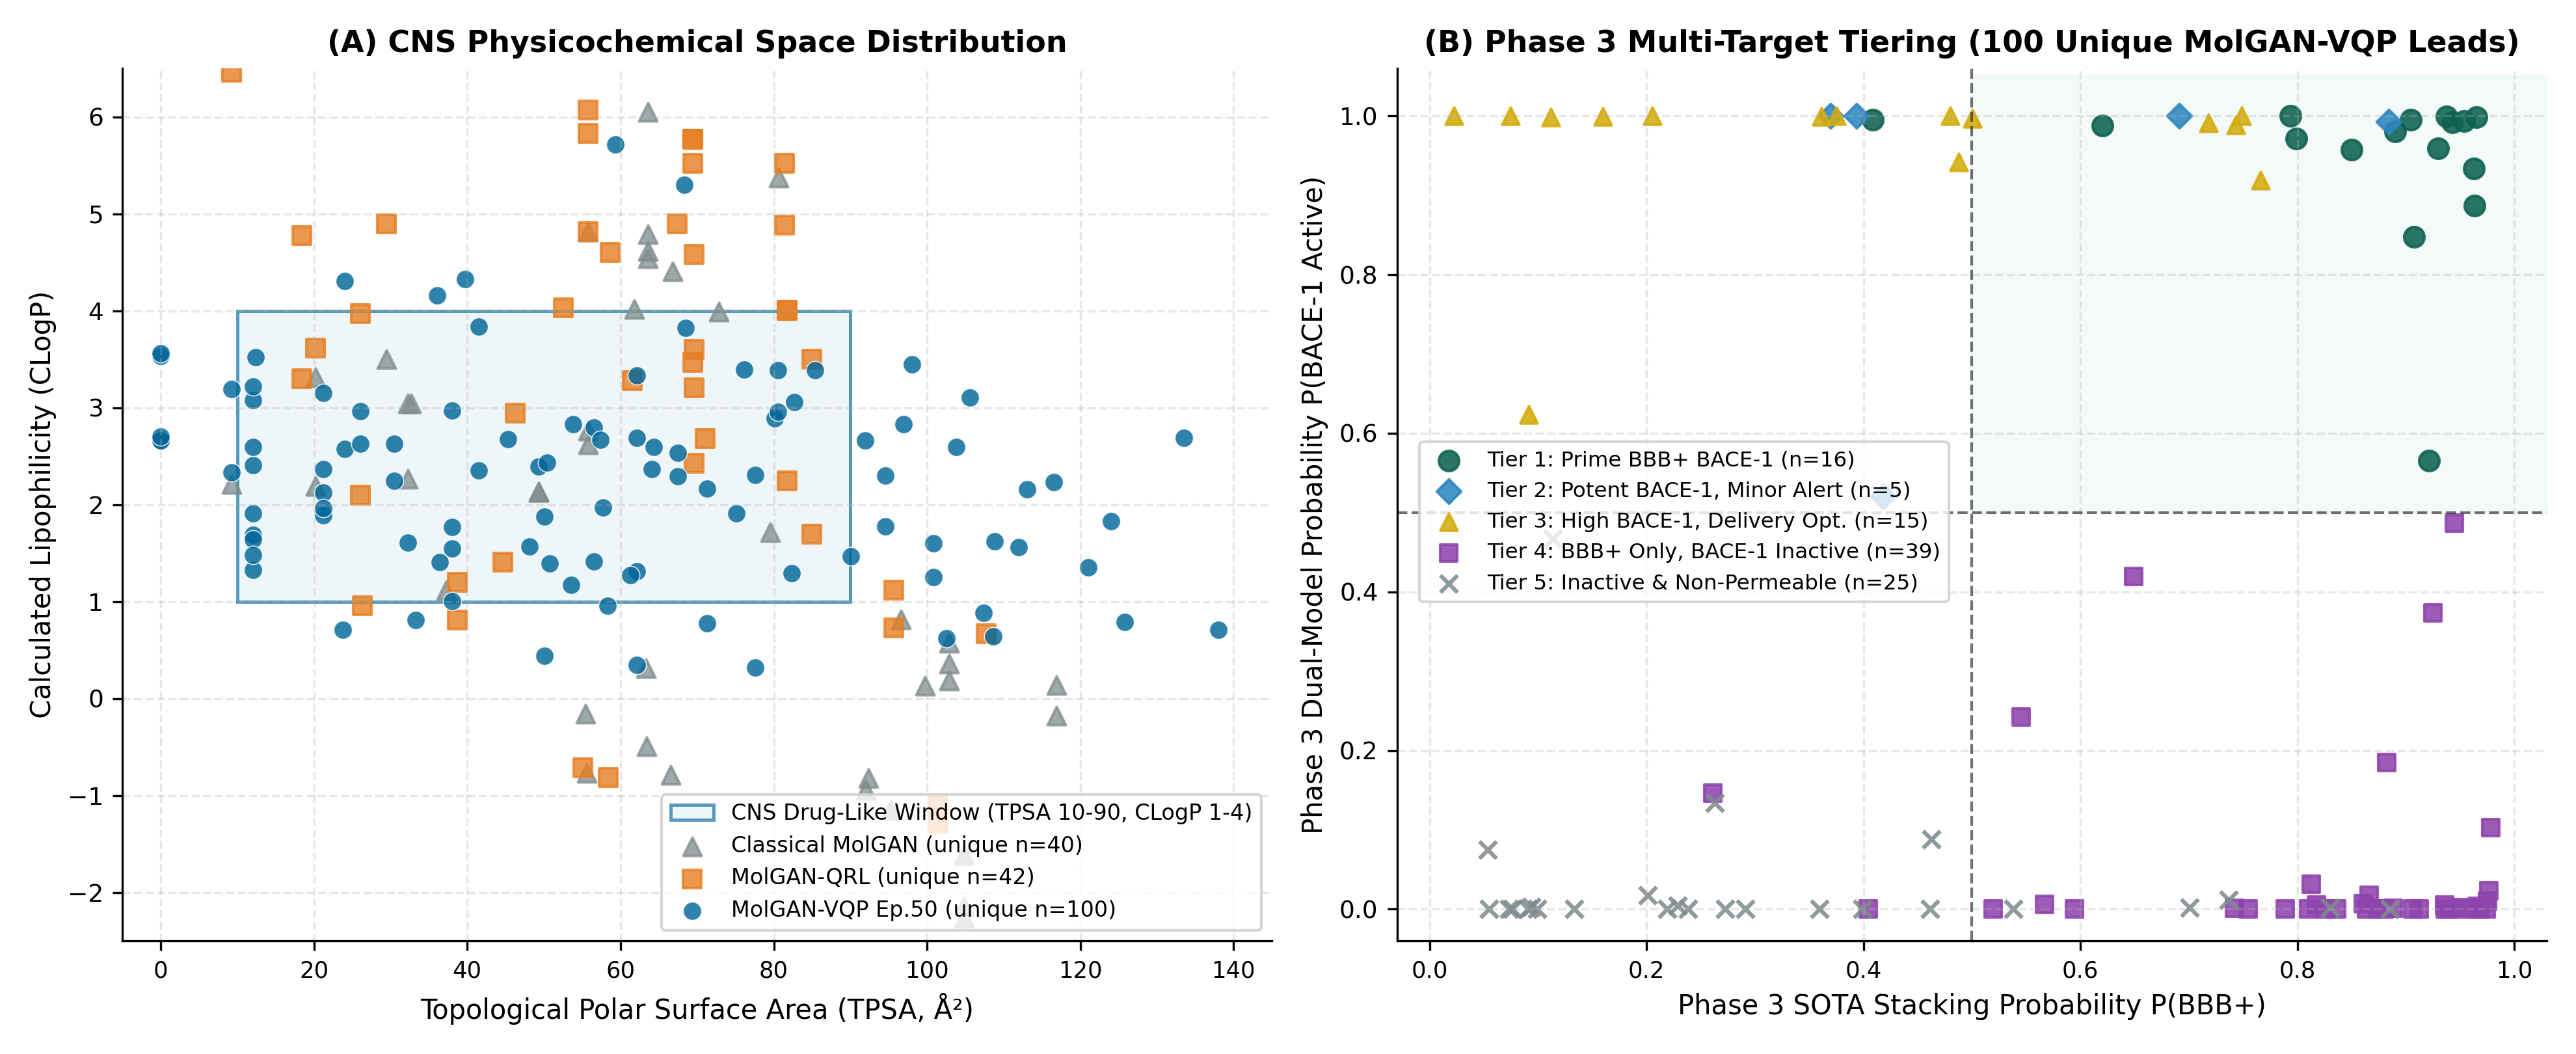
\includegraphics[width=\textwidth]{fig_cns_distributions.png}
\caption{Pharmacokinetic and multi-target distributions of the 100 unique Epoch-50 MolGAN-VQP candidates (\texttt{screened\_leads\_100\_vqp}): \textbf{(A)} TPSA versus CLogP relative to Classical MolGAN ($n=40$ unique) and MolGAN-QRL ($n=42$ unique), showing MolGAN-VQP enrichment within the CNS window; \textbf{(B)} Phase 3 multi-target screening stratification across SOTA stacking $P(\text{BBB}^+)$ and dual $P(\text{BACE-1})$ classifying leads into Tiers 1--5 ($16, 5, 15, 39, 25$).}
\label{fig:cns_dist}
\end{figure}

\subsection{Circuit Edge-Head Latency Benchmark and Quantum-Classical Comparison}
Because full state-vector simulation of sequential quantum bond selection incurs significant wall-clock latency over long molecular graphs ($N \le 35$), we benchmarked four architectural configurations of Phase 2 edge prediction (\texttt{ActorRGCN\_Jerbi}) alongside classical and quantum GAN baselines in Table~\ref{tab:edge_bench}. All variants preserve the 9-qubit \texttt{JerbiAtomPolicy} head while swapping only the pairwise bond selection circuit:
\begin{itemize}[noitemsep]
    \item \textbf{\texttt{edge=mlp} (Fast Hybrid Configuration, 96,058 Actor Params):} Retains the 9-qubit data re-uploading atom selector (19,062 params) paired with a $192 \to 128 \to 4$ classical edge MLP (25,220 params), running a 4-molecule rollout in \textbf{3.26 s} (enabling full 50-epoch training in 2.02 hours on a single RTX 2000 Ada GPU).
    \item \textbf{\texttt{edge=2q\_born} (\texttt{QuantumEdgePolicy2Q}, 6,261 Edge Params):} Encodes the four Kekul\'e bond orders directly into two-qubit Born-rule computational basis probabilities $|\langle b_0 b_1|\psi\rangle|^2$ ($\mathrm{P}(|00\rangle,\dots,|11\rangle)$), running 4 rollouts in \textbf{10.33 s}.
    \item \textbf{\texttt{edge=jerbi} (Dual-Quantum, 89,799 Actor Params):} Combines the 9-qubit \texttt{JerbiAtomPolicy} and 4-qubit \texttt{JerbiEdgePolicy} (18,961 edge params), taking \textbf{21.29 s} per 4-molecule rollout while yielding the highest BACE-1 (40.0\%), BBB+ (80.0\%), and Tier-1 (20.0\%) hit rates in our 20-molecule dual-quantum evaluation.
\end{itemize}

\begin{table}[!htbp]
\centering
\caption{Multi-model benchmark comparing Classical MolGAN (Strict \& Heuristic), MolGAN-QRL [2], the 4-qubit QM9 baseline, and MolGAN-VQP quantum circuit configurations.}
\label{tab:edge_bench}
\setlength{\tabcolsep}{4pt}
\footnotesize
\begin{tabularx}{\textwidth}{@{}>{\raggedright\arraybackslash}X cccccc@{}}
\toprule
\textbf{Model / Edge-Head Architecture} & \textbf{Generator} & \textbf{Uniq.} & \textbf{Clean} & \textbf{5/6-Ring} & \textbf{Tier-1} & \textbf{4-Mol} \\
 & \textbf{Type} & \textbf{(\%)} & \textbf{(\%)} & \textbf{(\%)} & \textbf{(\%)} & \textbf{Latency} \\
\midrule
Classical MolGAN (Heuristic / Strict) & 1-Shot MLP & 32.0 / 40.0 & 42.0 / 43.0 & 16.0 / 6.0 & 6.25 / 12.50 & $<0.1\text{ s}$ \\
MolGAN-QRL [2] (Heuristic / Strict) & 1-Shot MLP & 38.0 / 42.0 & 82.0 / 54.0 & 4.0 / 8.0 & 7.89 / 11.90 & $<0.1\text{ s}$ \\
MolGAN-QPolicy (4Q QM9 Baseline) & 4Q Autoreg. & 88.3 & 36.4 & 0.0 & 19.12* & --- \\
MolGAN-VQP (\texttt{9Q Atom + ClassicalEdge}) & 9Q + 1,580p MLP & --- & --- & --- & --- & --- \\
\rowcolor{lightgray}
MolGAN-VQP (\texttt{9Q Atom + MLP Edge}, 96,058p) & 9Q + 25.2k MLP & \textbf{100.0} & \textbf{99.0} & \textbf{90.0} & 16.00 & \textbf{3.26 s} \\
MolGAN-VQP (\texttt{9Q Atom + 2Q Born Edge}) & 9Q + 2Q Born & --- & --- & --- & --- & 10.33 s \\
\rowcolor{lightgray}
MolGAN-VQP Dual-Quantum (\texttt{9Q + 4Q}, 89,799p) & 9Q + 4Q Jerbi & \textbf{100.0} & 90.0 & 80.0 & \textbf{20.00} & 21.29 s \\
\bottomrule
\end{tabularx}
\end{table}

\subsection{Full-Scale 50-Epoch PPO Reinforcement Learning Dynamics}
The full-scale training run (\texttt{Results/\allowbreak full\_scale\_50epochs/\allowbreak 2026-11-11\_00-42-05/}, batch size $=16$, 50 epochs) completed in \textbf{7,280.94 seconds} (\textbf{2.02 hours}; $127.92$--$155.68\text{ s/epoch}$, mean $145.62\text{ s/epoch}$) on the 13,988-molecule CNS library. Training trajectories extracted directly from \texttt{metrics.csv} are shown in Figure~\ref{fig:training_curves}:
\begin{enumerate}[noitemsep]
    \item \textbf{Invariant Integrity \& Anti-Strain Stability (Fig.~\ref{fig:training_curves}A):} Chemical validity, uniqueness, and novelty remained locked at \textbf{100.0\%} across every single epoch 1--50, completely averting late-stage PPO collapse. Clean unstrained stability rose from $93.75\%$ at Epoch 1 to a 50-epoch mean of \textbf{97.88\%}, finishing at \textbf{100.0\%} at Epoch 50 (nearly doubling the pre-Rule-14 50.0\% stability baseline).
    \item \textbf{Actor-Critic Convergence (Fig.~\ref{fig:training_curves}B):} Critic value MSE decayed rapidly from $0.2757$ (Epoch 1) to a minimum of $0.0258$ (mean $0.0608$, ending at $0.0406$), while clipped surrogate actor loss remained well-regulated within $[-0.1430, -0.0434]$ (mean $-0.0775$).
    \item \textbf{Adversarial Discriminator Equilibrium (Fig.~\ref{fig:training_curves}C):} The R-GCN discriminator BCE loss transitioned smoothly from $0.5983$ to an equilibrium band around $0.4303$--$0.52$ (mean $0.5234$), providing steady graph-topology regularization without saturating gradients.
    \item \textbf{Multi-Objective Reward Trajectory (Fig.~\ref{fig:training_curves}D):} Composite reward remained strongly positive throughout training, peaking at \textbf{+0.7482} (Epoch 4, mean \textbf{+0.6289}) while balancing batch-mean $P(\text{BBB}^+)$ (mean $0.6187$, peak $0.8613$) and $P(\text{BACE-1})$ (mean $0.4487$, peak $0.6384$) under Murcko scaffold diversity pressure (bucket ceiling $25$).
\end{enumerate}

\begin{figure}[!htbp]
\centering
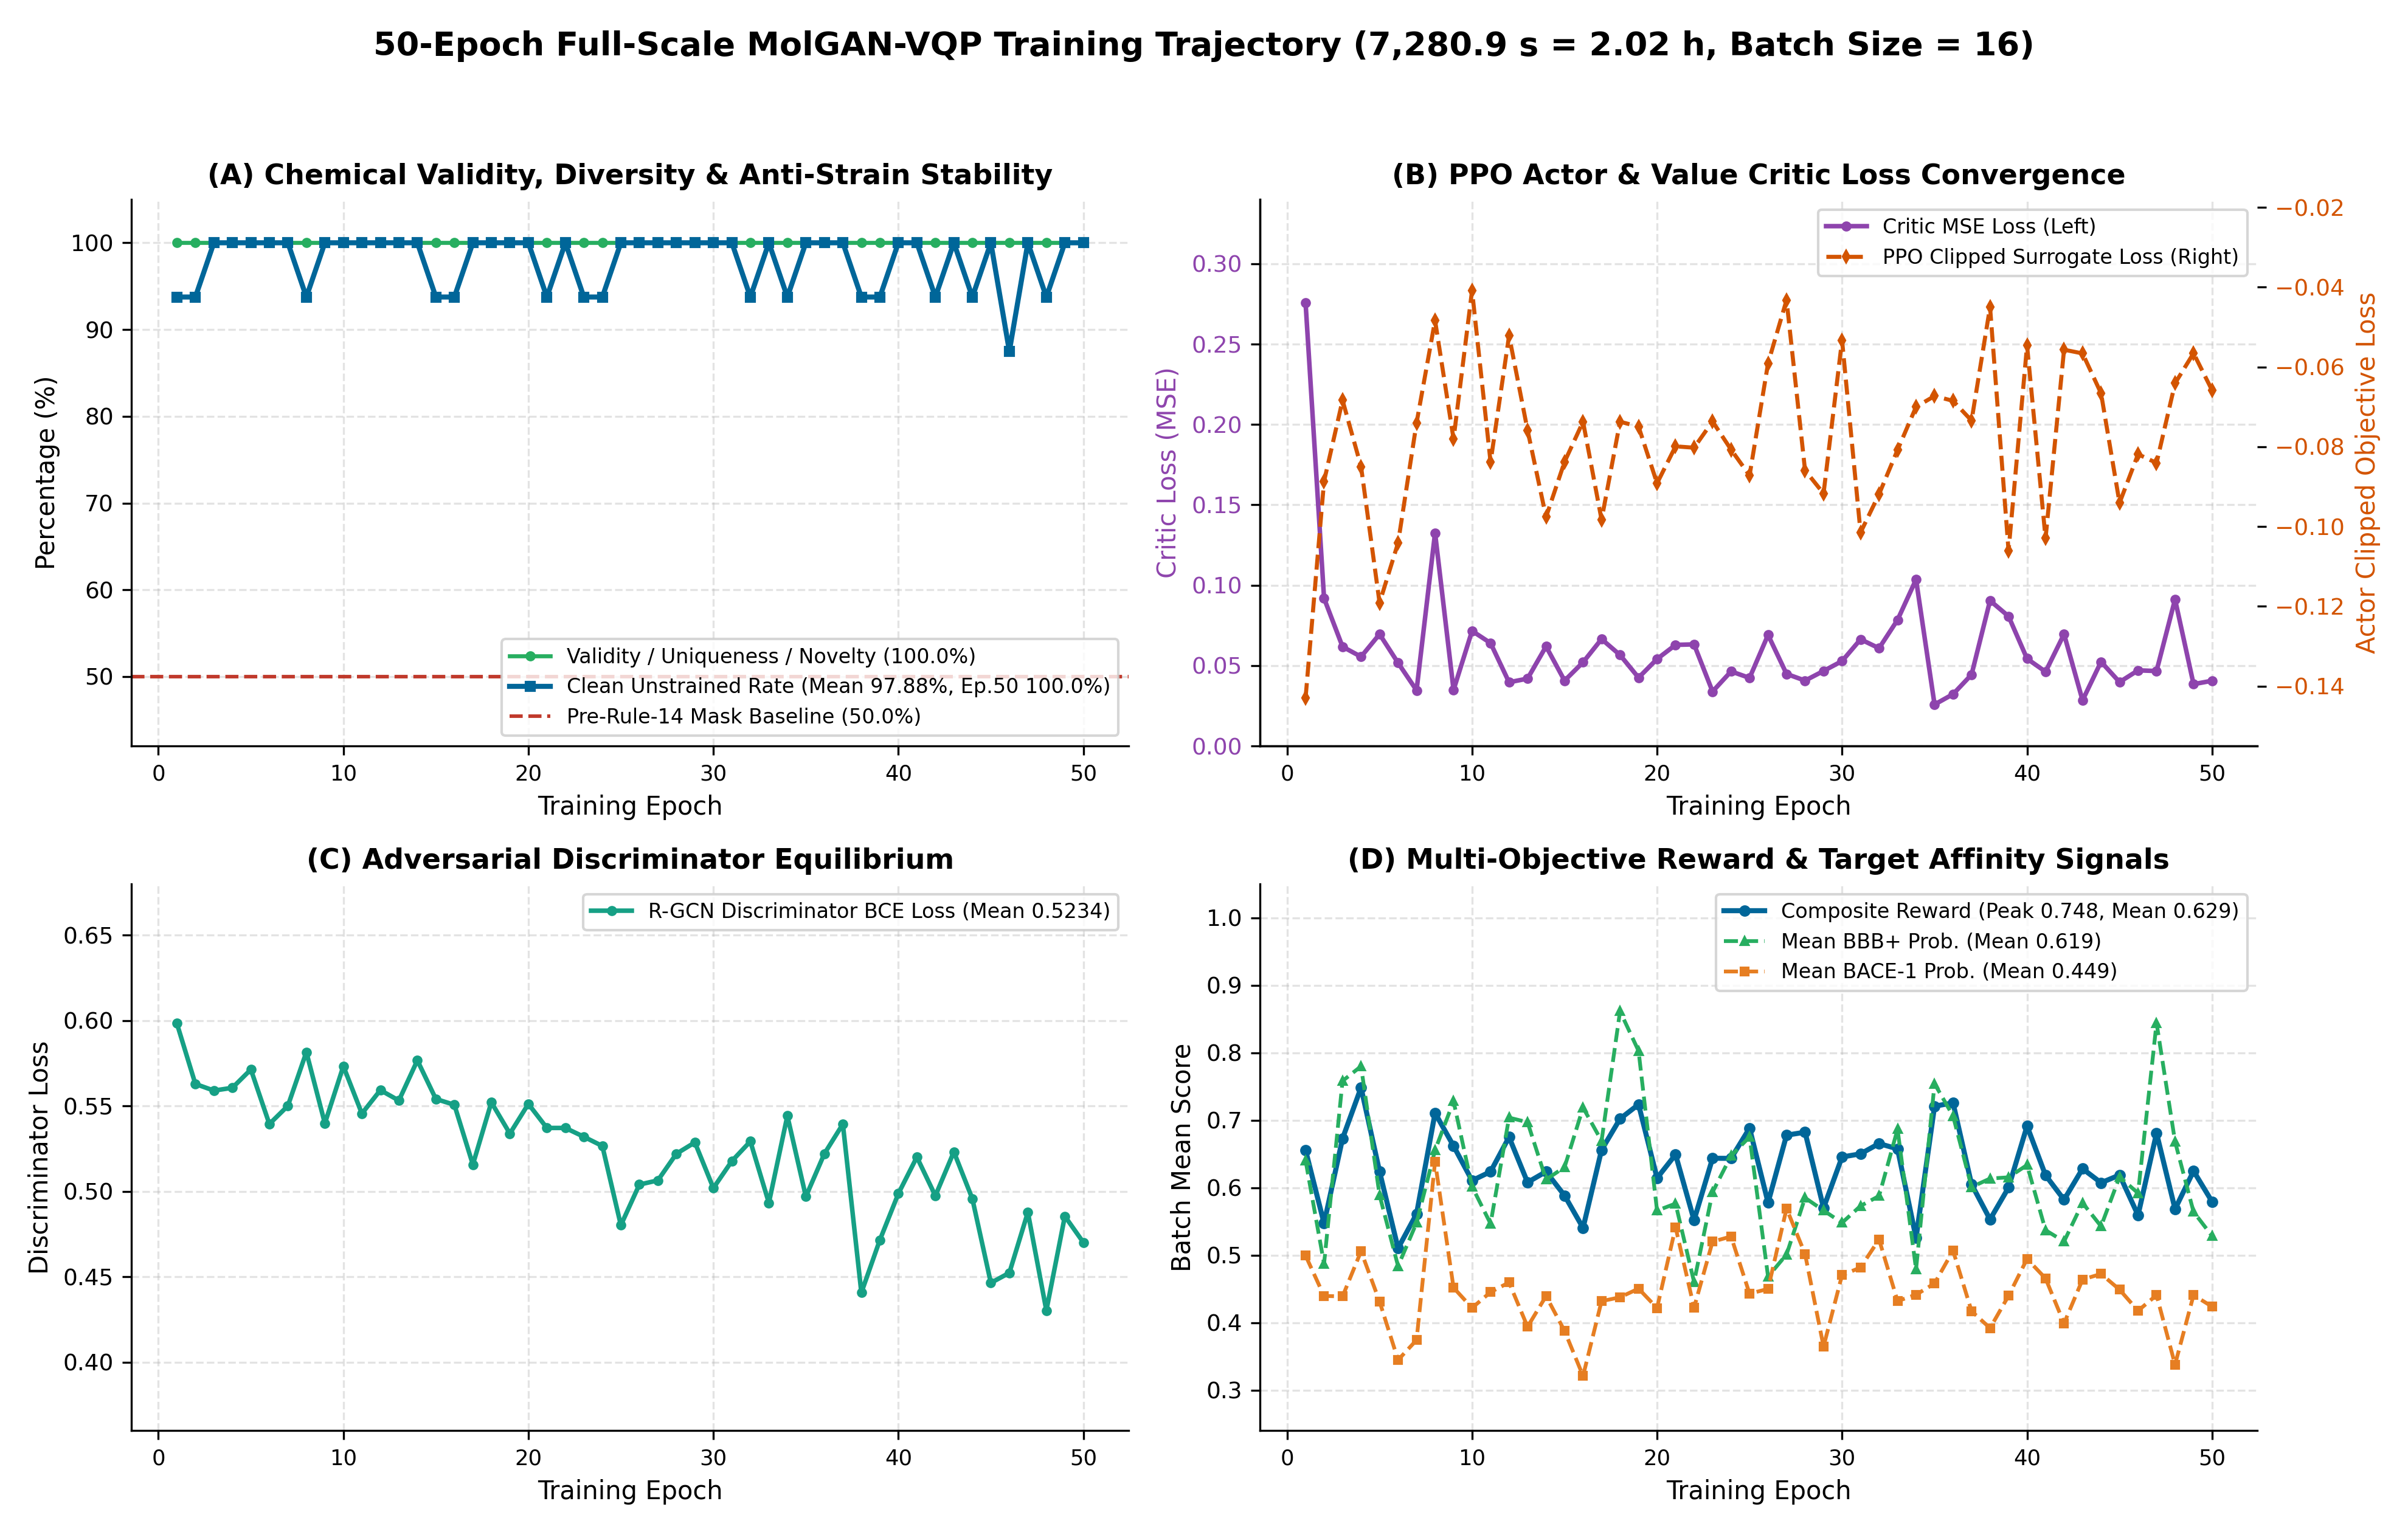
\includegraphics[width=\textwidth]{fig_training_curves.png}
\caption{Empirical 50-epoch training trajectories from \texttt{Results/\allowbreak full\_scale\_50epochs/\allowbreak 2026-11-11\_00-42-05/\allowbreak log\_dir/\allowbreak metrics.csv}: \textbf{(A)} Validity, uniqueness, novelty ($100.0\%$ invariant), and anti-strain stability ($97.88\%$ mean, $100.0\%$ Epoch 50 vs. $50.0\%$ pre-Rule-14 baseline); \textbf{(B)} Critic MSE loss ($0.2757 \to 0.0406$) and PPO clipped objective; \textbf{(C)} R-GCN discriminator equilibrium ($0.5983 \to 0.43$--$0.52$); and \textbf{(D)} Composite reward (peak $+0.748$) and target prediction curves.}
\label{fig:training_curves}
\end{figure}

\subsection{Component-Wise Ablation Studies}
To quantify the causal necessity of each safety and architectural layer in MolGAN-VQP, we evaluate controlled ablations on the trained 50-epoch checkpoint and compare against pre-upgrade baselines (Table~\ref{tab:ablations}):
\begin{itemize}[noitemsep]
    \item \textbf{Ablation 1 --- Removing Dynamic Valence Masking ($N=100$):} Disabling \texttt{compute\_valence\_mask} causes catastrophic chemical collapse: validity plunges immediately from $100.0\%$ to \textbf{0.0\%} ($0.0\%$ uniqueness, $0.0\%$ cleanliness) due to uncontrolled valence saturation and impossible bond multi-closures.
    \item \textbf{Ablation 2 --- Removing CNS Atom Caps ($N=100$, \texttt{ablation\_no\_atom\_filters.csv}):} Keeping dynamic valence rules active while removing element caps ($\mathrm{P}/\mathrm{I}$ hard ban, $\le 35\%$ heteroatoms, step-0 carbon start) maintains $100.0\%$ connectivity and $94.0\%$ uniqueness, yet \textbf{destroys cleanliness ($99.0\% \to \mathbf{0.0\%}$)}. The unconstrained policy generates isolated halogens ($\mathrm{I}$, $\mathrm{F}$), $\mathrm{P}/\mathrm{I}$ hyper-heteroatom rings such as \texttt{\seqsplit{FC(PC1SC(I)SC1F)C1SNC(C(P)I)P(S)S1}} ($\mathrm{MW}=655.24\text{ Da}, \mathrm{QED}=0.121$), halving QED ($0.412 \to 0.255$) and collapsing Tier-1 yield to \textbf{5.32\%}.
    \item \textbf{Ablation 3 --- Pre-Rule-14 Baseline (Without Bridged/Bredt/Cycle Strain Guards):} Earlier checkpoints trained prior to Rule-14 strict 5/6/7-ring and Bredt enforcement suffered high chemical strain, attaining only $50.0\%$ cleanliness in Epoch-1 training logs and $56.2\%$--$81.2\%$ in 16-molecule screens, versus $97.88\%$ mean / $100.0\%$ Epoch-50 cleanliness in the complete engine.
\end{itemize}

\begin{table}[!htbp]
\centering
\caption{Component-wise ablation benchmark isolating dynamic valence masking, CNS atom caps, Rule-14 ring-strain guards, and dual-quantum bond selection.}
\label{tab:ablations}
\setlength{\tabcolsep}{4pt}
\footnotesize
\begin{tabularx}{\textwidth}{@{}>{\raggedright\arraybackslash}X ccccccc@{}}
\toprule
\textbf{Architecture Configuration} & \textbf{Samples} & \textbf{Valid} & \textbf{Uniq.} & \textbf{Clean} & \textbf{5/6-Ring} & \textbf{QED} & \textbf{Tier-1} \\
 & \textbf{($n$)} & \textbf{(\%)} & \textbf{(\%)} & \textbf{(\%)} & \textbf{(\%)} & \textbf{Mean} & \textbf{(\% Uniq.)} \\
\midrule
Ablation: w/o Dynamic Valence Masking & 100 & \textbf{0.0} & 0.0 & 0.0 & 0.0 & --- & 0.00 \\
Ablation: w/o CNS Atom Caps & 100 & 100.0 & 94.0 & \textbf{0.0} & 55.0 & 0.255 & 5.32 \\
Pre-Rule-14 Baseline (Ep. 1 / 16-Eval) & 16 & 100.0 & 100.0 & 50.0--56.2 & 93.8* & --- & 18.75 \\
\rowcolor{lightgray}
\textbf{MolGAN-VQP Complete (9Q + Mask, Ep. 50)} & 100 & \textbf{100.0} & \textbf{100.0} & \textbf{99.0} & \textbf{90.0} & \textbf{0.412} & 16.00 \\
\rowcolor{lightgray}
\textbf{MolGAN-VQP Dual-Quantum (9Q + 4Q)} & 20 & \textbf{100.0} & \textbf{100.0} & 90.0 & 80.0 & 0.398 & \textbf{20.00} \\
\bottomrule
\end{tabularx}
\par\vspace{0.1cm}
\raggedright\footnotesize *Pre-Rule-14 16-molecule evaluation exhibited bridged/strained rings flagged as unstable (\texttt{Clean = 56.2\%}).
\end{table}

\section{Discussion}

\subsection{Resolving Mode Collapse via Quantum Data Re-Uploading and Structural Constraints}
Comparing MolGAN-QRL [2] ($42.0\%$ strict uniqueness, $8.0\%$ stable 5/6-membered rings) against MolGAN-VQP ($100.0\%$ uniqueness, $90.0\%$ stable 5/6-membered rings) clarifies why quantum placement inside a generator matters fundamentally. When a VQC merely scores dense one-shot matrices [2], policy gradients still contend with quadratic $\mathcal{O}(N^2)$ edge relaxations; the generator minimizes variance by collapsing onto a handful of repetitive chains or bloated macrocycles. In MolGAN-VQP, pairing autoregressive graph construction with Jerbi-style data re-uploading circuits [51] injects state representations repeatedly into $R_Y$ encoding angles interspersed with circular CNOT entanglers across all 9 element registers and 4 bond registers. Simultaneously, Phase 1 FiLM conditioning provides each trajectory with a distinct structural anchor $\mathbf{z} \in \mathbb{R}^{32}$ from continuous manifold space, while the Murcko scaffold counter prevents reward dominance by any single motif.

\subsection{Interplay Between Deterministic Masking and Policy Gradients}
Critically, quantum expressivity without chemical grammar fails just as dramatically when physical constraints are removed (Ablation 1: $0.0\%$ validity; Ablation 2: $0.0\%$ cleanliness). Conversely, deterministic masking alone cannot generate Alzheimer's therapeutics: random masked rollouts without policy shaping frequently miss BACE-1 pharmacophores or optimal CNS-MPO balance. By zeroing unphysical logits ($\mathrm{O}{-}\mathrm{O}$, $\mathrm{N}{-}\mathrm{N}$, bridged cages, $\mathrm{C}{=}\mathrm{S}$, and $>7$-membered macrocycles) \textit{before} Softmax sampling, PPO gradient variance is restricted strictly to the subspace of valid, clean, synthesizable Kekul\'e graphs. This explains why MolGAN-VQP reaches $100.0\%$ validity from Epoch 1 while converging smoothly over 50 epochs.

\subsection{Translational Pharmacology and Expanded Dataset Calibration}
A pivotal finding during development was that earlier BACE-1 classifiers trained on smaller or noisier datasets exhibited poor out-of-distribution generalization ($0.6433$ OOD ROC-AUC). Expanding our dual Phase 3 bioactivity dataset from 4,669 to \textbf{14,972 records} (11,825 harmonized BindingDB \texttt{P56817} + ChEMBL \texttt{CHEMBL4822} molecules thresholded at $\le 100\text{ nM}$ with $94.71\%$ overlap concordance) elevated held-out BACE-1 test discrimination to \textbf{0.9242 ROC-AUC}, alongside expanding the unsupervised CNS structural library to \textbf{21,508 molecules} ($+7,520$ curated BACE-1 ligands). The resulting Tier-1 leads in Table~\ref{tab:flagship_leads} combine compact bicyclic heteroatom cores, strategic $\mathrm{F}/\mathrm{Cl}$ bioisosteres blocking metabolic oxidation, primary/secondary amines suited for aspartate dyad interactions, and low polar surface area favorable for passive BBB transit.

\subsection{Limitations and Future Directions}
Several limitations define clear avenues for next-generation work. First, raw RDKit SAS across the 100-molecule campaign averaged $5.74 \pm 0.59$ (median $5.86$), reflecting saturated bridgehead-adjacent substituents; incorporating retrosynthetic accessibility penalties or reaction-template actions should lower SAS below $4.5$. Second, our Phase 2 circuits were evaluated via noiseless PennyLane state-vector backpropagation (\texttt{default.qubit}), where sequential 4-qubit bond circuits run $6.5\times$ slower than hybrid MLP edge heads ($21.29\text{ s}$ vs. $3.26\text{ s}$ per 4 molecules). Compiling trained 9-qubit and 4-qubit circuits onto NISQ superconducting/ion-trap processors using parameter-shift gradients and validating flagship Tier-1 leads via 3D molecular docking inside X-ray crystal structures (e.g., PDB BACE-1 complexes) and MD/MM-GBSA free-energy simulations represent immediate pre-synthetic priorities.

\section{Conclusion}
We presented \textbf{MolGAN-VQP}, a unified 3-phase framework uniting GraphVAE latent FiLM conditioning, dual Jerbi-style data re-uploading quantum policies (9-qubit atom selection and 4-qubit bond order prediction), a deterministic 14-rule anti-strain and valence masking engine, and calibrated multi-modal BBB/BACE-1 screening for Alzheimer's drug design. By replacing brittle one-shot matrix generation with quantum-guided autoregressive construction, MolGAN-VQP eliminates mode collapse ($40\%$--$42\% \to \mathbf{100.0\%}$ uniqueness), elevates strain-free chemical cleanliness to \textbf{99.0\%} ($100.0\%$ at Epoch 50), increases stable 5/6-membered ring drug topologies to \textbf{90.0\%}, and discovers unique, novel, brain-penetrant BACE-1 active leads achieving $P(\text{BBB}^+) \le 0.966$, $P(\text{BACE-1}) \le 1.000$, and Pfizer $\text{CNS-MPO} \le 5.25$.

\section{Methods}

\subsection{Chemical Libraries and Graph Data Preprocessing}
The primary CNS training dataset comprises \textbf{13,988 curated brain-relevant small molecules} spanning $9 \le N \le 35$ heavy atoms (used for the 50-epoch full-scale PPO benchmark), subsequently expanded by $+7,520$ BACE-1 inhibitors to \textbf{21,508 structures} in \texttt{cns\_alzheimers\_9\_35.sparsedataset}. Molecular graphs are Kekulized natively in RDKit with all explicit aromatic bond orders converted into localized alternating single/double bonds across \textbf{4 discrete bond channels}: $e \in \{0:\text{None}, 1:\text{Single}, 2:\text{Double}, 3:\text{Triple}\}$. Heavy atoms span \textbf{10 element channels} (index $0$ padding + 9 chemical symbols): $\{1:\mathrm{C}(4), 2:\mathrm{N}(3), 3:\mathrm{O}(2), 4:\mathrm{F}(1), 5:\mathrm{I}(1), 6:\mathrm{P}(5), 7:\mathrm{S}(2), 8:\mathrm{Cl}(1), 9:\mathrm{Br}(1)\}$.

\subsection{Phase 1: GraphVAE Encoder and Continuous FiLM Conditioning}
Phase 1 employs a \texttt{GraphVAE} ($6,111,555$ parameters, $N_{\max}=35, |E|=4, |\mathcal{V}|=10, \mathbf{z} \in \mathbb{R}^{32}$). Its \texttt{GraphEncoder} stacks two degree-normalized Relational GCN layers ($10 \to 128 \to 64$) with $\text{LeakyReLU}(0.2)$ activations, soft attention-gated global pooling $\mathbf{a} = \sigma(\mathbf{W}_{\text{att}}\mathbf{H})$, linear projection ($64 \to 128$), and Gaussian variational heads ($\boldsymbol{\mu}, \log\boldsymbol{\sigma}^2 \in \mathbb{R}^{32}$). In a 500-sample diagnostic evaluation of the standalone Phase 1 checkpoint (\texttt{vae\_model.pt}), the classical one-shot decoder achieved $79.19\%$ atom-type accuracy and $95.62\%$ edge accuracy, but only \textbf{14.0\% (70/500)} full-molecule chemical validity---quantifying one-shot decoding fragility at $N=35$. Accordingly, MolGAN-VQP freezes only the \texttt{GraphEncoder} and transfers sampled $\mathbf{z} \in \mathbb{R}^{32}$ into Phase 2 via Feature-wise Linear Modulation (FiLM):
\begin{equation}
[\boldsymbol{\gamma} \,\|\, \boldsymbol{\beta}] = \mathrm{LeakyReLU}(\mathbf{W}_{\text{FiLM}}\mathbf{z} + \mathbf{b}_{\text{FiLM}}) \in \mathbb{R}^{128}, \qquad \mathbf{h}_G' = (1 + \tanh\boldsymbol{\gamma}) \odot \mathbf{h}_G + \boldsymbol{\beta} \in \mathbb{R}^{64}.
\end{equation}

\subsection{Phase 2: Dual Data Re-Uploading Quantum Policies and 14-Rule Masking}

\subsubsection*{9-Qubit Atom Prediction PQC (\texttt{JerbiAtomPolicy})}
At step $t$, \texttt{JerbiAtomPolicy} ($19,062$ parameters) assigns one qubit exclusively to each heavy element ($\mathrm{Q}_0$--$\mathrm{Q}_8$). Across $L=3$ variational blocks, classical state features $\mathbf{h}_G' \in \mathbb{R}^{64}$ are re-uploaded at every layer $l \in \{0, 1, 2\}$ via dedicated $\text{MLP}_l$ subnetworks ($64 \to 64 \to 9$) outputting $\boldsymbol{\alpha}^{(l)} = \pi \tanh(\mathrm{MLP}_l(\mathbf{h}_G')) \in [-\pi, \pi]^9$:
\begin{equation}
|\psi_{\text{atom}}(\mathbf{h}_G'; \boldsymbol{\theta})\rangle = \prod_{l=0}^{L-1} \left[ \left(\bigotimes_{i=0}^{8} \mathrm{Rot}(\theta_{l,i,0}, \theta_{l,i,1}, \theta_{l,i,2})\right) \left(\prod_{i=0}^{8} \mathrm{CNOT}_{(i, (i+1)\bmod 9)}\right) \left(\bigotimes_{i=0}^{8} R_Y(\alpha_i^{(l)})\right) \right] |0\rangle^{\otimes 9}.
\end{equation}
Measured Pauli-$Z$ expectation values $\langle Z_i \rangle \in [-1, 1]$ are scaled by a learnable temperature weight $\beta_{\text{atom}}$ (initialized at $3.0$), combined with covalent geometry compatibility modulation $\mathbf{x}_{\text{compat}}$ (measuring closeness to $\mathrm{C}=1.911$, $\mathrm{N}=1.866$, $\mathrm{O}/\mathrm{S}=1.824$, $\mathrm{P}=1.745$ affinities plus anti-$\mathrm{N}{-}\mathrm{N}$, anti-$\mathrm{O}{-}\mathrm{O}$, anti-$\mathrm{S}{-}\mathrm{S}$, and Carbon-tethered halogen rules) and CNS atom caps before Softmax sampling: step $0$ forced to Carbon, hard exclusion of $\mathrm{P}$ and $\mathrm{I}$, halogen mutual exclusivity, $\mathrm{S} \le 1$, heteroatom cap $\le \max(2, \lfloor 0.35\, N_{\text{target}} \rfloor)$, and $\mathrm{C}_{\text{frac}} \ge 0.65$ after step 3.

\subsubsection*{4-Qubit Bond Prediction PQC (\texttt{JerbiEdgePolicy})}
For each candidate pair $(u, v)$ linking newly added atom $u$ to existing atom $v < u$, the edge policy takes concatenated pair representations $\mathbf{f}_{u,v} = [\mathbf{h}_u \,\|\, \mathbf{h}_v \,\|\, \mathbf{h}_G'] \in \mathbb{R}^{192}$. In \texttt{JerbiEdgePolicy} ($18,961$ parameters), $\mathbf{f}_{u,v}$ is re-uploaded over $L=3$ layers ($192 \to 32 \to 4$) across 4 dedicated bond wires ($\mathrm{Q}_0$: No Bond, $\mathrm{Q}_1$: Single, $\mathrm{Q}_2$: Double, $\mathrm{Q}_3$: Triple) with circular 4-qubit CNOT entanglement and $\mathrm{Rot}(\boldsymbol{\varphi}_{l,k})$ gates. Scaled readout logits $\beta_{\text{edge}}\langle Z_k\rangle$ are gated by the deterministic mask $\mathcal{M}_{\text{val}}(u, v) \in \{0, -\infty\}^4$. Notice we also evaluated a compact 2-qubit Born-rule circuit (\texttt{QuantumEdgePolicy2Q}, $6,261$ params), a minimal classical circuit emulator (\texttt{ClassicalEdgeCircuit}, $1,580$ params), and a fast MLP head ($25,220$ params, totaling $96,058$ actor parameters vs. $89,799$ in the dual-quantum actor).

\subsubsection*{Deterministic 14-Rule Dynamic Valence and Anti-Strain Masking Engine}
Prior to sampling each bond order $b \in \{0,1,2,3\}$, \texttt{compute\_valence\_mask} enforces 14 exact graph-theoretic and chemical rules: (1) padding veto, (2) monovalent halogens restricted to single-bond Carbon only, (3) ban on mixed geminal halogens and $\text{CF}_3$ bursts, (4) ban on direct $\mathrm{O}{-}\mathrm{O}$ peroxides, (5) ban on $\mathrm{N}{-}\mathrm{N}$ hydrazines/triazenes and $\mathrm{N}{-}\mathrm{O}$ hydroxylamines, (6) ban on $\mathrm{S}{-}\mathrm{S}$ disulfides, (7) ban on $\mathrm{C}{=}\mathrm{S}$ thiones, (8) exact remaining atomic valence capacity $\min(\mathrm{Val}_{\max}(u)-\mathrm{val}_u, \mathrm{Val}_{\max}(v)-\mathrm{val}_v)$, (9) global triple-bond cap $\le 1$, (10) cumulene prevention ($\mathrm{X}{=}\mathrm{C}{=}\mathrm{Y}$), (11) backward bond cap $\le 2$ per added atom, (12) cyclomatic ring budget $\le 2$ ($e - v + 1 \le 2$), (13) strict shortest-path cycle closure filter allowing \textbf{only 5-, 6-, or 7-membered rings} (path length $\ge 4$ edges), anti-bridged-cage check ($\le 2$ shared cycle edges), and anti-cycloalkyne protection, and (14) dynamic Bredt's rule banning double bonds at bridgehead atoms or strained exocyclic ring junctions.

\subsubsection*{PPO Optimization and Hierarchical Composite Reward}
Episodic rollouts stored in \texttt{PPOBuffer} use full molecular return $R(G)$ with direct episodic advantages $\hat{A}_t = R(G) - V_\phi(s_t)$ standardized across each training batch, optimized via clipped PPO [43] ($\epsilon = 0.2$, $4$ update epochs, entropy coefficient $c_{\text{ent}} = 0.10$):
\begin{equation}
\mathcal{L}^{\text{CLIP}}(\theta) = \hat{\mathbb{E}}_t\left[\min\left(\rho_t(\theta)\hat{A}_t,\, \mathrm{clip}(\rho_t(\theta), 1-\epsilon, 1+\epsilon)\hat{A}_t\right)\right] + c_{\text{ent}}\mathcal{H}(\pi_\theta).
\end{equation}
The terminal composite reward (\texttt{CompositeRewardCalculator}, bounded in $[-1.0, +1.0]$) integrates target predictions, synthetic tractability, adversarial realism, SMARTS strain penalties, and Murcko scaffold novelty:
\begin{equation}
R(G) = \mathrm{clip}\Big(\big[ 0.45\,P(\text{BACE-1}) + 0.30\,P(\text{BBB}^+) + 0.15\,r_{\text{SAS}} + 0.10\,\sigma(D(G)) + b_{\text{bonus}} - p_{\text{strain}} \big] \cdot \gamma_{\text{C}} \cdot (1 - s_{\max}^2) \cdot f_{\text{Murcko}},\ -1, 1\Big),
\end{equation}
where $b_{\text{bonus}}$ rewards active bioactivity ($\ge 0.5$), BBB permeation ($\ge 0.5$), $\mathrm{SAS} \le 3.5$, and 1--2 clean 5/6-membered rings ($-0.10$ if acyclic); $p_{\text{strain}}$ penalizes reactive SMARTS instability motifs ($0.30$ per violation); $\gamma_{\text{C}}=\min(1, c_{\text{frac}}/0.65)$; $s_{\max}$ penalizes nearest-neighbor Tanimoto similarity; and $f_{\text{Murcko}}$ decays linearly once a scaffold exceeds bucket size $25$. Alongside the actor/critic, a 9-qubit \texttt{QuantumPhysChemEvaluator} ($81$ parameters) encodes continuous RDKit properties into auxiliary quantum descriptors.

\subsection{Phase 3: Multi-Modal Screening and Experimental Setup}
Phase 3 triages generated molecules through two calibrated predictors and automated CNS-MPO [14, 15] tiering:
\begin{itemize}[noitemsep]
    \item \textbf{BBB Permeation Stacking Ensemble (\texttt{bbb\_sota}):} Trained on 8,456 curated molecules using Bemis-Murcko scaffold splits over a \textbf{2,233-dimensional} RDKit descriptor vector ($2,048$-bit ECFP4 + $166$ MACCS keys + $19$ CNS/physicochemical descriptors) plus $24$-D atom node features in \texttt{MolGCN}. Combining fixed blend weights $0.35\,\hat{p}_{\text{LGBM}} + 0.45\,\hat{p}_{\text{XGB}} + 0.10\,\hat{p}_{\text{DeepCNSNet}} + 0.10\,\hat{p}_{\text{MolGCN}}$ yields a held-out scaffold test \textbf{0.9632 ROC-AUC}, $0.9775$ PR-AUC, $90.20\%$ accuracy, $91.98\%$ sensitivity, $87.31\%$ specificity, and $0.7924$ MCC.
    \item \textbf{Expanded Dual BACE-1/BBB Classifier (\texttt{bace1\_dual}):} Uses $2,058$-D molecular features ($2,048$ Morgan ECFP4 + $10$ normalized physicochemical properties) through a $2058 \to 512 \to 256$ shared MLP trunk with twin $64 \to 1$ prediction heads. Trained on an expanded \textbf{14,972-record} dataset unifying 11,825 harmonized BindingDB (\texttt{P56817}) and ChEMBL (\texttt{CHEMBL4822}) BACE-1 ligands ($\mathrm{IC}_{50}/K_i \le 100\text{ nM}$ active cutoff, $94.71\%$ cross-database overlap concordance) with 3,152 BBB records, achieving \textbf{0.9242 held-out BACE-1 ROC-AUC} ($85.5\%$ accuracy) and \textbf{0.9481 BBB ROC-AUC}.
\end{itemize}
All models were executed using \textbf{Python 3.8.20}, \textbf{PyTorch 2.0.1+cu118}, \textbf{PennyLane 0.20.0} (\texttt{default.qubit} with adjoint/backprop differentiation), and \textbf{RDKit 2020.09.1} on an \textbf{NVIDIA RTX 2000 Ada Generation GPU (16,380 MiB VRAM, Driver 580.178.04)}. Key optimization hyperparameters: batch size $16$, $\text{lr}_{\text{actor}} = 10^{-4}$, $\text{lr}_{\text{critic}} = 10^{-3}$, $\text{lr}_{\text{disc}} = 10^{-4}$, PPO epochs $4$, $\epsilon = 0.2$, entropy $c_{\text{ent}} = 0.10$, and scaffold bucket size $25$. Performance was quantified via Validity, Uniqueness, Novelty, Internal Morgan Tanimoto Diversity, NVU, Strain-Free Clean Rate, Stable 5/6-Ring Yield, QED [44], SAS [45], NP/ADMET metrics [46, 47], and CNS-MPO [14, 15].

\section*{Declarations}
\subsubsection*{Acknowledgments}
The authors acknowledge departmental GPU computing infrastructure and open-source chemical bioactivity repositories from ChEMBL and BindingDB.

\subsubsection*{Author Contributions}
M.M., Y.N.M., and M.K. conceptualized the 3-phase MolGAN-VQP architecture, implemented the dual Jerbi data re-uploading quantum policies, dynamic 14-rule valence masking engine, and Phase 3 target screening pipelines, performed all empirical benchmarks and ablation analyses, and wrote and approved the final manuscript.

\subsubsection*{Competing Interests}
The authors declare that they have no competing financial or non-financial interests.

\subsubsection*{Availability of Data and Materials}
Source code, trained Phase 1/2/3 checkpoints, expanded BACE-1/CNS datasets, and evaluation CSVs are maintained in the project workspace (\texttt{molgan\_vqp/}, \texttt{phase1\_autoencoder/}, \texttt{phase3\_testing\_models/}) extending the baseline repository \url{https://github.com/Ihebhergli22/MolGAN-QRL} and \url{https://github.com/Yukesh-Naren/MOlGAN-VQP}.

\subsubsection*{Funding}
This research was supported by departmental computing and laboratory resources.

% ==============================================================================
% REFERENCES
% ==============================================================================
\begin{thebibliography}{51}
\small
\setlength{\itemsep}{0.4pt}
\setlength{\parskip}{0pt}

\bibitem{1} S. Ashenden, ``Introduction to drug discovery,'' in \textit{The Era of Artificial Intelligence, Machine Learning, and Data Science in the Pharmaceutical Industry}, Academic Press, pp. 1--18, 2021. \url{https://doi.org/10.1016/B978-0-12-820045-2.00002-7}
\bibitem{2} M. I. Hergli and E. Harigua-Souiai, ``MolGAN-QRL: a hybrid framework for molecule generation using quantum-enhanced reinforcement learning,'' \textit{Journal of Cheminformatics}, vol. 16, no. 1, p. 42, 2024. \url{https://doi.org/10.1186/s13321-024-00835-1}
\bibitem{3} N. Berdigaliyev and M. Aljofan, ``An overview of drug discovery and development,'' \textit{Future Medicinal Chemistry}, vol. 12, no. 10, pp. 939--947, 2020. \url{https://doi.org/10.4155/fmc-2019-0307}
\bibitem{4} T. Hwang, et al., ``Failure of investigational drugs in late-stage clinical development and publication of trial results,'' \textit{JAMA Internal Medicine}, vol. 176, no. 12, pp. 1826--1833, 2016. \url{https://doi.org/10.1001/jamainternmed.2016.6008}
\bibitem{5} M. Gu, et al., ``Forward or backward: lessons learned from small molecule drugs approved by FDA from 2012 to 2022,'' \textit{Molecules}, vol. 28, no. 24, p. 7941, 2023. \url{https://doi.org/10.3390/molecules28247941}
\bibitem{6} J. Cummings, et al., ``Alzheimer's disease drug development pipeline: 2023,'' \textit{Alzheimer's \& Dementia: Translational Research \& Clinical Interventions}, vol. 9, no. 2, p. e12385, 2023. \url{https://doi.org/10.1002/trc2.12385}
\bibitem{7} D. He, et al., ``De novo generation and identification of novel compounds with drug efficacy based on machine learning,'' \textit{Advanced Science}, vol. 11, no. 12, p. 2307245, 2024. \url{https://doi.org/10.1002/advs.202307245}
\bibitem{8} D. J. Selkoe and J. Hardy, ``The amyloid hypothesis of Alzheimer's disease at 25 years,'' \textit{EMBO Molecular Medicine}, vol. 8, no. 6, pp. 595--608, 2016. \url{https://doi.org/10.15252/emmm.201606210}
\bibitem{9} R. Vassar, et al., ``$\beta$-Secretase cleavage of Alzheimer's amyloid precursor protein by the transmembrane aspartic protease BACE,'' \textit{Science}, vol. 286, no. 5440, pp. 735--741, 1999. \url{https://doi.org/10.1126/science.286.5440.735}
\bibitem{10} A. K. Ghosh, et al., ``BACE1 inhibitors for Alzheimer's disease: active site specificity and catalytic mechanism,'' \textit{Journal of Medicinal Chemistry}, vol. 55, no. 17, pp. 7445--7469, 2012. \url{https://doi.org/10.1021/jm300438q}
\bibitem{11} P. C. May, et al., ``The potent BACE1 inhibitor LY2886721 fails to progress due to liver toxicity in Phase II clinical trials,'' \textit{Journal of Neuroscience}, vol. 35, no. 3, pp. 1199--1210, 2015. \url{https://doi.org/10.1523/JNEUROSCI.4129-14.2015}
\bibitem{12} N. J. Abbott, et al., ``Structure and function of the blood-brain barrier,'' \textit{Neurobiology of Disease}, vol. 37, no. 1, pp. 13--25, 2010. \url{https://doi.org/10.1016/j.nbd.2009.07.030}
\bibitem{13} W. A. Banks, ``From blood-brain barrier to blood-brain interface: new opportunities for CNS drug delivery,'' \textit{Nature Reviews Drug Discovery}, vol. 15, no. 4, pp. 275--292, 2016. \url{https://doi.org/10.1038/nrd.2015.21}
\bibitem{14} T. T. Wager, X. Hou, P. R. Verhoest, and A. Villalobos, ``Moving beyond rules: the development of a central nervous system multiparameter optimization (CNS MPO) approach to enable alignment of drug-like properties,'' \textit{ACS Chemical Neuroscience}, vol. 1, no. 6, pp. 435--449, 2010. \url{https://doi.org/10.1021/cn100008x}
\bibitem{15} T. T. Wager, et al., ``Central nervous system multiparameter optimization desirabilities: design principles for brain-penetrant therapeutics,'' \textit{ACS Chemical Neuroscience}, vol. 7, no. 6, pp. 767--775, 2016. \url{https://doi.org/10.1021/acschemneuro.6b00029}
\bibitem{16} G. Sittampalam, et al., ``Mapping biologically active chemical space to accelerate drug discovery,'' \textit{Nature Reviews Drug Discovery}, vol. 18, no. 2, pp. 83--84, 2018. \url{https://doi.org/10.1038/d41573-018-00007-2}
\bibitem{17} W. Warr, et al., ``Exploration of ultralarge compound collections for drug discovery,'' \textit{Journal of Chemical Information and Modeling}, vol. 62, no. 9, pp. 2021--2034, 2022. \url{https://doi.org/10.1021/acs.jcim.2c00224}
\bibitem{18} Y. Bian and X. Xie, ``Generative chemistry: drug discovery with deep learning generative models,'' \textit{Journal of Molecular Modeling}, vol. 27, no. 3, p. 71, 2021. \url{https://doi.org/10.1007/s00894-021-04674-8}
\bibitem{19} D. P. Kingma and M. Welling, ``Auto-encoding variational Bayes,'' in \textit{International Conference on Learning Representations (ICLR)}, 2014. \url{https://arxiv.org/abs/1312.6114}
\bibitem{20} I. Goodfellow, et al., ``Generative adversarial nets,'' in \textit{Advances in Neural Information Processing Systems (NeurIPS)}, vol. 27, pp. 2672--2680, 2014.
\bibitem{21} R. G\'omez-Bombarelli, et al., ``Automatic chemical design using a data-driven continuous representation of molecules,'' \textit{ACS Central Science}, vol. 4, no. 2, pp. 268--276, 2018. \url{https://doi.org/10.1021/acscentsci.7b00572}
\bibitem{22} M. Olivecrona, et al., ``Molecular de-novo design through deep reinforcement learning,'' \textit{Journal of Cheminformatics}, vol. 9, no. 1, p. 48, 2017. \url{https://doi.org/10.1186/s13321-017-0235-x}
\bibitem{23} B. S\'anchez-Lengeling, et al., ``Optimizing distributions over molecular space: an objective-reinforced generative adversarial network for inverse-design chemistry (ORGANIC),'' \textit{ChemRxiv}, 2017. \url{https://doi.org/10.26434/chemrxiv.5309668}
\bibitem{24} L. Yu, et al., ``SeqGAN: sequence generative adversarial nets with policy gradient,'' in \textit{AAAI Conference on Artificial Intelligence}, vol. 31, no. 1, pp. 2852--2858, 2017.
\bibitem{25} T. Kipf and M. Welling, ``Semi-supervised classification with graph networks,'' in \textit{International Conference on Learning Representations (ICLR)}, 2017.
\bibitem{26} M. Schlichtkrull, et al., ``Modeling relational data with graph convolutional networks,'' in \textit{The Semantic Web (ESWC)}, pp. 593--607, 2018. \url{https://doi.org/10.1007/978-3-319-93417-4_38}
\bibitem{27} W. Jin, R. Barzilay, and T. Jaakkola, ``Junction tree variational autoencoder for molecular graph generation,'' in \textit{International Conference on Machine Learning (ICML)}, pp. 2323--2332, 2018.
\bibitem{28} C. Shi, et al., ``GraphAF: a flow-based autoregressive model for molecular graph generation,'' in \textit{International Conference on Learning Representations (ICLR)}, 2020.
\bibitem{29} J. You, et al., ``Graph convolutional policy network for goal-directed molecular graph generation,'' in \textit{Advances in Neural Information Processing Systems (NeurIPS)}, vol. 31, pp. 6410--6421, 2018.
\bibitem{30} E. J. Jang, S. Gu, and B. Poole, ``Categorical reparameterization with Gumbel-softmax,'' in \textit{International Conference on Learning Representations (ICLR)}, 2017.
\bibitem{31} N. De Cao and T. Kipf, ``MolGAN: an implicit generative model for small molecular graphs,'' in \textit{ICML Workshop on Theoretical Foundations and Applications of Deep Generative Models}, 2018. \url{https://arxiv.org/abs/1805.11973}
\bibitem{32} Z. Jiang, et al., ``Mode collapse alleviation of reinforcement learning-based GANs in drug design,'' in \textit{IEEE International Conference on Bioinformatics and Biomedicine (BIBM)}, pp. 3045--3052, 2023. \url{https://doi.org/10.1109/BIBM58861.2023.10385948}
\bibitem{33} J. Zou, et al., ``STAGAN: an approach to improve the stability of molecular graph generation based on generative adversarial networks,'' \textit{Computers in Biology and Medicine}, vol. 167, p. 107691, 2023. \url{https://doi.org/10.1016/j.compbiomed.2023.107691}
\bibitem{34} J. Biamonte, et al., ``Quantum machine learning,'' \textit{Nature}, vol. 549, no. 7671, pp. 195--202, 2017. \url{https://doi.org/10.1038/nature23474}
\bibitem{35} M. Schuld and F. Petruccione, \textit{Supervised Learning with Quantum Computers}, Springer, 2018.
\bibitem{36} P.-H. Wang, et al., ``Recent advances in quantum computing for drug discovery and development,'' \textit{IEEE Nanotechnology Magazine}, vol. 17, no. 2, pp. 26--30, 2023. \url{https://doi.org/10.1109/MNANO.2023.3249499}
\bibitem{37} J. Li, R. O. Topaloglu, and S. Ghosh, ``Quantum generative models for small molecule drug discovery,'' \textit{IEEE Transactions on Quantum Engineering}, vol. 2, pp. 1--8, 2021. \url{https://doi.org/10.1109/TQE.2021.3104804}
\bibitem{38} P.-Y. Kao, et al., ``Exploring the advantages of quantum generative adversarial networks in generative chemistry,'' \textit{Journal of Chemical Information and Modeling}, vol. 63, no. 11, pp. 3307--3318, 2023. \url{https://doi.org/10.1021/acs.jcim.3c00562}
\bibitem{39} M. Anoshin, et al., ``Hybrid quantum cycle generative adversarial network for small molecule generation,'' \textit{IEEE Transactions on Quantum Engineering}, vol. 5, pp. 1--14, 2024. \url{https://doi.org/10.1109/TQE.2024.3414264}
\bibitem{40} R. Ramakrishnan, et al., ``Quantum chemistry structures and properties of 134 kilo molecules,'' \textit{Scientific Data}, vol. 1, p. 140022, 2014. \url{https://doi.org/10.1038/sdata.2014.22}
\bibitem{41} T. P. Lillicrap, et al., ``Continuous control with deep reinforcement learning,'' in \textit{International Conference on Learning Representations (ICLR)}, 2016.
\bibitem{42} M. Arjovsky, S. Chintala, and L. Bottou, ``Wasserstein generative adversarial networks,'' in \textit{International Conference on Machine Learning (ICML)}, pp. 214--223, 2017.
\bibitem{43} J. Schulman, F. Wolski, P. Dhariwal, A. Radford, and O. Klimov, ``Proximal policy optimization algorithms,'' \textit{arXiv preprint arXiv:1707.06347}, 2017.
\bibitem{44} G. R. Bickerton, et al., ``Quantifying the chemical beauty of drugs,'' \textit{Nature Chemistry}, vol. 4, no. 2, pp. 90--98, 2012. \url{https://doi.org/10.1038/nchem.1243}
\bibitem{45} P. Ertl and A. Schuffenhauer, ``Estimation of synthetic accessibility score of drug-like molecules based on molecular complexity and fragment contributions,'' \textit{Journal of Cheminformatics}, vol. 1, no. 1, p. 8, 2009. \url{https://doi.org/10.1186/1758-2946-1-8}
\bibitem{46} P. Ertl, et al., ``Natural product-likeness score and its application for prioritization of compound libraries,'' \textit{Journal of Chemical Information and Modeling}, vol. 48, no. 1, pp. 68--74, 2008. \url{https://doi.org/10.1021/ci700286x}
\bibitem{47} L. Guan, et al., ``ADMET-score: a comprehensive scoring function for evaluation of chemical drug-likeness,'' \textit{MedChemComm}, vol. 10, no. 1, pp. 148--157, 2019. \url{https://doi.org/10.1039/C8MD00472B}
\bibitem{48} A. M. Thomas, et al., ``QCA-MolGAN: Quantum circuit associative molecular GAN with multi-agent reinforcement learning,'' in \textit{IEEE International Conference on Quantum Artificial Intelligence (QAI)}, 2025. \url{https://doi.org/10.1109/QAI63978.2025.00029}
\bibitem{49} D. F. Veber, et al., ``Molecular properties that influence the oral bioavailability of drug candidates,'' \textit{Journal of Medicinal Chemistry}, vol. 45, no. 12, pp. 2615--2623, 2002. \url{https://doi.org/10.1021/jm020017n}
\bibitem{50} C. A. Lipinski, et al., ``Experimental and computational approaches to estimate solubility and permeability in drug discovery and development settings,'' \textit{Advanced Drug Delivery Reviews}, vol. 46, no. 1--3, pp. 3--26, 2001. \url{https://doi.org/10.1016/S0169-409X(00)00129-0}
\bibitem{51} S. Jerbi, C. Gyurik, S. Marshall, H. Briegel, and V. Dunjko, ``Parametrized quantum policies for reinforcement learning,'' in \textit{Advances in Neural Information Processing Systems (NeurIPS)}, vol. 34, pp. 28362--28375, 2021.
\end{thebibliography}

\end{document}
